\chapter{Bahnoptimierung}
%\cite{Eggers.2019}
%\cite{Engelke.2008}
%\cite{Ziaukas.2017}
%\cite{Hansen.2012}
%\cite{Spong.2020}
%
\section{Definition des Optimierungsproblems}
Gegenstand der Optimierung ist die Minimierung des Energieverbrauchs eines KR210 R2700-2 Industrieroboters entlang einer Bewegungsbahn. Im Ziel der Arbeit ist festgelegt, den Ansatz möglichst praktikabel für die Automobilproduktion zu gestalten. Dazu wird der Begriff der Bewegungsbahn weiter eingegrenzt. Es wird unterschieden zwischen prozessbezogenen Bewegungen, z.B. entlang einer Schweißnaht oder Klebebahn, und nicht-prozessbezogenen Bewegungen, z.B. das Anfahren einer Vorposition oder der Home-Position in der Bewegungsart PTP. Im Folgenden werden explizit nicht prozessrelevante Trajektorien betrachtet. Der Ansatz basiert auf der geometrischen Anpassung  der Bewegungsbahn durch einen zu optimierenden Parametervektor $\bm{q}_{v}$. Dieser umfasst die Gelenkwinkel des, nach der Hälfte der Bewegungsdauer definierten Via-Punkts \cite[S~532~ f.]{Ziaukas.2017}.
%
\begin{equation}
	\label{eqn:parametervektor}
	\bm{q}_{v} = [q_{v,1},...,q_{v,6}]^T 
\end{equation}
%
Der Startwert jedes Via-Punkts wird auf der Hälfte der Winkelposition zwischen dem Start- und Zielpunkt definiert.
\begin{equation}
	\label{eqn:parametervektor-startkonfiguration}
	q_{v,i,Start} = \dfrac{q_{s,i}+q_{e,i}}{2} ~\forall~ i \in \{1,...,6\}
\end{equation}
Die Minimierung der Leistungsaufnahme basiert auf der konfigurationsabhängigen Reduktion der Massenträgheitsmomente in $\bm{M}(\bm{q})$, so dass bei gleichbleibender Winkelbeschleunigung die Drehmomente in den Gelenken reduziert werden \cite[S.~531]{Ziaukas.2017}. Das Optimierungsproblem besteht darin, den Parametervektor zu identifizieren, für den die minimale Zielfunktion erreicht wird.
%\begin{equation}
%	\bm{q}_{v,opt} = \argminA_{\bm{q}_{v}} J_{P_{zu}}(\bm{q}_{v}).
%\end{equation}
%
\begin{equation}
	\argminA_{\bm{q}_{v}} J(\bm{q}_{v}) = \{\bm{q}_{v} \mid J(\bm{q}_{v}) = \min_{\bm{q}_{v,opt}} J(\bm{q}_{v,opt})\}.
\end{equation}
%
\section{Zielfunktion}
Für die Definition der Zielfunktion wird angenommen, dass die generatorisch erzeugte Leistung während des Abbremsvorgangs über Bremswiderstände dissipiert \cite[S.~1327]{Pellicciari.2015}. Zur Identifizierung des Optimums werden die Zielfunktionen \ref{eqn:torque}, \ref{eqn:emechges} \cite[S.~1216]{Saravanan.2008} und \ref{eqn:emech} \cite[S.~57]{Eggers.2019} aufgestellt. Die Integrationsgrenzen $t_s$ und $t_e$ entsprechen dem Start- bzw. Zielzeitpunkt. Der Ausdruck \ref{eqn:torque} wird in abgewandelter Form in \cite[S-~1]{Hansen.2012} beschrieben und erzielt durch Quadrieren den Vorteil, dass hohe Drehmomente stärker gewichtet werden. Dabei wird jedoch nicht ersichtlich, ob Leistung aufgenommen oder abgegeben wird.
%
\begin{equation}
	\label{eqn:torque}
	J_{\tau}(\bm{q}_{v}) = \int_{ts}^{te}\sum_{i=1}^{n}\tau_i(t)^2~dt
\end{equation}
%
Von einem Vorschlag der Zielfunktion \ref{eqn:emechges} wird ebenso Abstand genommen, da hierbei die generatorisch umgewandelte Leistung während des Abbremsvorgangs als aufgenommene Leistung der Verbraucher bewertet wird. 
%
\begin{equation}
	\label{eqn:emechges}
	J_{P_{mech_{ges}}}(\bm{q}_{v}) = \int_{ts}^{te}\sum_{i=1}^{n}\left|\tau_i(t)\dot{q_i}\right|^2~dt
\end{equation}
%
Die Zielfunktion \ref{eqn:emech} entspricht dem physikalischen Ausdruck der verrichteten mechanischen Arbeit über die zugeführte Leistung. Es wird ausschließlich die motorisch aufgenommene, mechanische Leistung $P_{mech}>0$ berücksichtigt. 
%
\begin{equation}
	\label{eqn:emech}
	J_{P_{mech_{zu}}}
	(\bm{q}_{v}) 
	= E_{mech}(\bm{q}_{v}) 
	=\int_{ts}^{te}P_{mech_{zu}}(\bm{q}_{v},t)~dt
\end{equation}
%
Die numerische Implementierung der Zielfunktion in  MATLAB\textsuperscript{\textregistered} entspricht der Gleichung  \ref{eqn:numerischezielfunktion}. Die Schrittweite ist in Anlehnung an die Abtastung der Messeinrichtung  mit $\Delta t = 0.004 \text{s}$ festgelegt. Die Anzahl der Schritte $m$  wird gemäß $(t_s-t_e)/\Delta t$ berechnet.
%
\begin{equation}
	\label{eqn:numerischezielfunktion}
	J_{P_{mech_{zu}}}
	(\bm{q}_{v}) 
	= E_{mech}(\bm{q}_{v}) 
	= \sum_{k=1}^{m} P_{mech_{zu}}(\bm{q}_{v},t)~\Delta t
\end{equation}
%
\section{Nebenbedingungen}
Die Verfahrzeit bleibt gegenüber der Initialbahn konstant und wird durch den Zielzeitpunkt $t_e$ vorgegeben. 
%Eine Anpassung der Variablen für die maximale relative Geschwindigkeit $vel axis[i]$ und Maximalbeschleunigung $acc axis[i]$ im KRL Programm siehe \cite[S.~532]{Ziaukas.2017} erfolgt nicht.
In \cite[S.~40]{Eggers.2019} bzw. \cite[S.~5]{Hansen.2012} werden die Gelenkwinkel der energie-optimalen Bewegungsbahn in der Robotersteuerung über einen Software-in-the-Loop (SiL) Ansatz berechnet. Dadurch ist die Einhaltung von Drehmoment-, Gelenkwinkel-, Geschwindigkeit- und Beschleunigungsgrenzen entsprechend der Gleichungen \ref{eqn:conpos},\ref{eqn:convel}, \ref{eqn:conacc} und \ref{eqn:contau} gewährleistet. 
%
\begin{equation}
	\label{eqn:conpos}
	q_{i,min} \leq q_{i}(t) \leq q_{i,max}  ~\forall~ i \in \{1,...,6\}
\end{equation}
%
\begin{equation}
	\label{eqn:convel}
	\dot{q}_{i,min} \leq \dot{q}_{i}(t) \leq \dot{q}_{i,max}  ~\forall~ i \in \{1,...,6\}
\end{equation}
%
\begin{equation}
	\label{eqn:conacc}
	\ddot{q}_{i,min} \leq \ddot{q}_{i}(t) \leq \ddot{q}_{i,max}  ~\forall~ i \in \{1,...,6\}
\end{equation}
%
\begin{equation}
	\label{eqn:contau}
	\tau_{i,min} \leq \tau_{i}(t) \leq \tau_{i,max}  ~\forall~ i \in \{1,...,6\}
\end{equation}
%
In der vorliegenden Arbeit sind ausschließlich die Schranken der Gelenkwinkel $q_{v,i}$ im Via-Punkt definiert. Die Formulierung zielt darauf ab, dass die optimierte Bewegungsbahn nicht signifikant von der Initialbahn abweicht \cite[S.~5]{Hansen.2012}.
\begin{equation}
	\label{eqn:Schranken}
	q_{v,i} \in [q_{i,min};q_{i,max}] ~\forall~ i \in \{1,...,6\}
\end{equation}
Grenzwerte für die Drehmomente, Winkelgeschwindigkeiten und Winkelbeschleunigungen werden nicht explizit formuliert.  Im Anschluss an die Optimierung erfolgt eine manuelle Überprüfung der Verläufe.
%
\section{Solver- und Optimierungsalgorithmus}
Die numerische Umsetzung der Optimierung erfolgt unter Verwendung der MATLAB\textsuperscript{\textregistered} Optimization Toolbox\texttrademark. Für das nichtlineare Optimierungsproblem wird anhand einer Entscheidungstabelle in \cite[S.~80]{OptimizationToolbox.2023} der Solver fmincon ausgewählt.  Im Anhang \ref{add:optimierer} ist der implementierte Code aufgeführt. Die Zielfunktion wird mithilfe des inversen Dynamik-Modells in der separaten MATLAB\textsuperscript{\textregistered}-Funktion $calc\_objective(qs,qe,qv,te)$ berechnet, siehe Anhang \ref{add:zielfunktion}. Es sind keine Gleichungs- bzw. Ungleichungssnebenbedingungen definiert. Es ist jedoch möglich, die im letzten Abschnitt beschriebenen Nebenbedingungen zu einem späteren Zeitpunkt hinzuzufügen. Für die einzelnen Via-Punkte des Parametervektors $\bm{q}_{v}$ sind jeweils die obere und untere Schranke entsprechend der Gleichung \ref{eqn:Schranken} festgelegt. Für den Algorithmus wird das Verfahren der sequentiellen quadratischen Programmierung (sequential quadratic programming (SQP)) gewählt.  SQP ist eine Verallgemeinerung des Newton-Verfahren\footnote{Das Newton-Verfahren ist ein numerischer Ansatz zur Lösung nichtlinearer Gleichungssysteme, bei dem eine iterative Approximation mithilfe der nach ersten Glied abgebrochenen Taylorreihe erfolgt \cite[S.~46]{Papageorgiou.2015}.} für beschränkte Problemstellungen \cite[S.~113]{Papageorgiou.2015}. In \cite[S.~253]{OptimizationToolbox.2023} wird beschrieben, dass für jeden Iterationsschritt die Einhaltung der Schranken gewährleistet ist. Diese wird als Vorteil aufgrund der Komplexität  der Inversen-Dynamik zur Berechnung der Zielfunktion  bewertet. Notwendige Bedingungen zur Identifikation eines lokalen Minimums sind die  Karush-Kuhn-Tucker (KKT) Konvergenzkriterien  \cite[S.~321]{Nocedal.2006}.  In jeder Iteration des SQP-Verfahrens wird versucht, die KKT-Bedingungen für das ursprüngliche Problem durch eine quadratische Approximation der Zielfunktion zu erfüllen \cite[S.~337~ff.]{Reinhardt.2013}. Zusätzlich bietet MATLAB\textsuperscript{\textregistered} für fmincon die Option, Konvergenzkriterien zu definieren. Im Rahmen der ersten KKT Bedingung wird der Gradient der Zielfunktion überprüft. Falls dieser Wert nur annähernd Null erreicht, kann ein Schwellenwert festgelegt werden, bei dessen Unterschreitung die erste KKT-Bedingung erfüllt ist. Es ist außerdem möglich, eine maximale Anzahl von Iterationen festzulegen, bei deren Erreichen der Algorithmus beendet wird. Die Variable \lstinline[language=Matlab]|'MaxIterations'| wird mit 25 frei gewählt.  Für eine ausführliche Herleitung von SQP-Algorithmen auf der Basis des Newton-Lagrange-Verfahren wird auf \cite[S.~529~ff.]{Nocedal.2006} verwiesen.








\section{Durchführung der Optimierung}
% todo bereits voerher Erwähnen?
Die Arbeit verfolgt den Anspruch, dass die identifizierten Einsparungen über das Laborumfeld hinaus in der industriellen Praxis realisiert werden können. Dazu wird eine Bewegung der Bewegungsart PTP betrachtet, die in nahezu jedem Programm den Verfahrweg nach Programmende in die Grundstellung abbildet. Exemplarisch wird die Fahrt vom letzten Prozesspunkt zurück in die Grundstellung im Fertigungsprogramm  $Kleben-Seitenwand$  optimiert. Diese wurde bereits im Kapitel Trajektorie-Planung \ref{sec:trajektorie} eingeführt. Die Start- und Zielkonfiguration ist in der Tabelle \ref{tab:simu} aufgeführt.  Im ersten Schritt wird die Initial-Trajektorie abgefahren. Dabei werden die Bewegungsdaten über die RSI-Signalaufzeichnung erfasst. Anhand der Genlenkwinkelgeschwindigkeitsverläufe, siehe Abbildung \ref{fig:winkelgeschwindigkeit_py1} wird die Gesamtbewegungsdauer mit 1,2 s geschätzt. Für die Startwerte \ref{eqn:parametervektor-startkonfiguration} des Parametervektors \ref{eqn:parametervektor} wird die Optimierung in MATLAB\textsuperscript{\textregistered}, siehe Anhang \ref{acc:optimierer} ausgeführt. Die Anzahl der Iterationen ist auf 25 beschränkt. In der Abbildung \ref{fig:funktionswerte-iteration} wird deutlich, dass die energie-optimalen Gelenkwinkel bereits nach acht Iterationsschritten näherungsweise erreicht sind.
%
\begin{figure}[tbph]
	\centering
	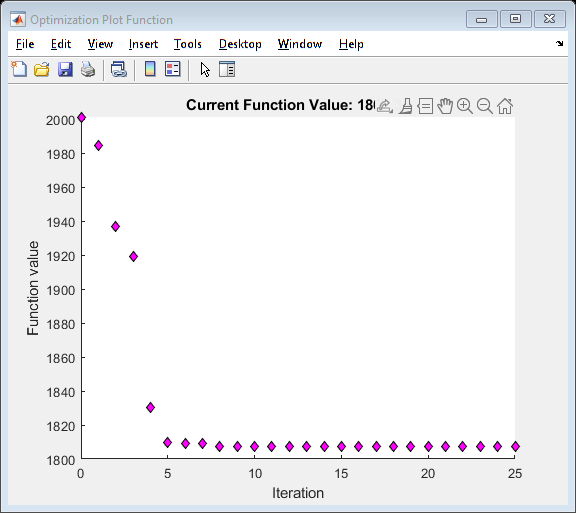
\includegraphics [width=4in]{images/optimization_01}
	\caption{Zielfunktionswerte einzelner Optimierungsiterationen}
	\label{fig:funktionswerte-iteration}
\end{figure}
%
\section{Auswertung der Optimierungsergebnisse}
Die identifizierten, energie-optimalen Via-Punkte sind in der Tabelle \ref{tab:optviapunkte} aufgeführt. Auffällig ist, dass für $q_{v,3}$ und $q_{v,4}$ die obere Schranke aktiv ist, sowie für $q_{v,6}$ die untere Schranke d. h. der Gelenkwinkel im Via-Punkt liegt auf dem selben Wert wie der Gelenkwinkel im Start- bzw. Zielpunkt. Für den Gelenkwinkel $q_{v,5}$ wird festgehalten, dass dieser auffällig nah am unteren Grenzwert liegt. Daraus folgt, dass die berechnete Trajektorie für die Gelenkwinkel drei, vier und sechs Werte außerhalb des Intervalls $[q_{i,s};q_{i,e}] ~\forall~ i \in \{3,4,5,6\}$ annimmt. 
\\
\begin{table}[tbph]
	\centering
	\caption{Winkelangaben letzter Prozesspunkt und Home-Position PRG $Kleben-Seitenwand$}
	\label{tab:optviapunkte}
	\begin{tabular}{|l|l|l|}
		\hline
		Startwert Gelenkwinkel&  Zielwert Gelenkwinkel&  Via-Punkte\\
		\hline
		$q_{s,1} = -53,8$			&  $q_{e,1} = -7,6^{\circ}$  		&$q_{v,1} = -25^{\circ}$  \\
		\hline
		$q_{s,2} = -70,3^{\circ}$	&  $q_{e,2} = -119,3^{\circ}$    	&$q_{v,2} = -96,1^{\circ}$  \\
		\hline
		$q_{s,3} = 98,8^{\circ}$	&  $q_{e,3} = 88,5^{\circ}$ 		&$q_{v,3} = 98,8^{\circ}$  \\
		\hline
		$q_{s,4} = -69,9^{\circ}$	&  $q_{e,4} = 10,3^{\circ}$ 		&$q_{v,4} = 10,3^{\circ}$  \\
		\hline
		$q_{s,5} = -58,7^{\circ}$	&  $q_{e,5} = 32,4^{\circ}$  		&$q_{v,5} = -47,1^{\circ}$  \\
		\hline
		$q_{s,6} = 55,7^{\circ}$	&  $q_{e,6} = -10,2^{\circ}$ 		&$q_{v,6} = -10,2^{\circ}$  \\
		\hline
	\end{tabular}
\end{table}
\\
Abbildung \ref{fig:popt} zeigt den Verlauf der mechanischen Leistung für die initiale Bewegungsbahn (ausgefüllte Linien) und den optimierten Leistungsverlauf (gestrichelte Linien). Wie erwartet, erzielt die Optimierung im Wesentlichen eine Energieeinsparung für das zweite Gelenk. Der simulierte mechanische Energieverbrauch des Roboters für die Initialbahn beträgt 2001 Joule. Die optimierte Bewegungsbahn wird mit einem mechanischen Energieverbrauch von 1807 Joule simuliert. Damit wird eine Energieeinsparung von ca. 9,7 \% prognostiziert. Für das erste Gelenk ist qualitativ einer Verschiebung des Bewegungsablaufs um 0,04 s nach nach links erkennbar. Des Weiteren ist eine geringfügige Zunahme der maximalen Leistungsaufnahme erkennbar. Für die Gelenke drei bis sechs sind minimale Abweichungen erkennbar, die aufgrund ihrer Größenordnung keinen signifikanten Einfluss auf die Energieeinsparung nehmen. 
%
\begin{figure}[tbph]
	\centering
	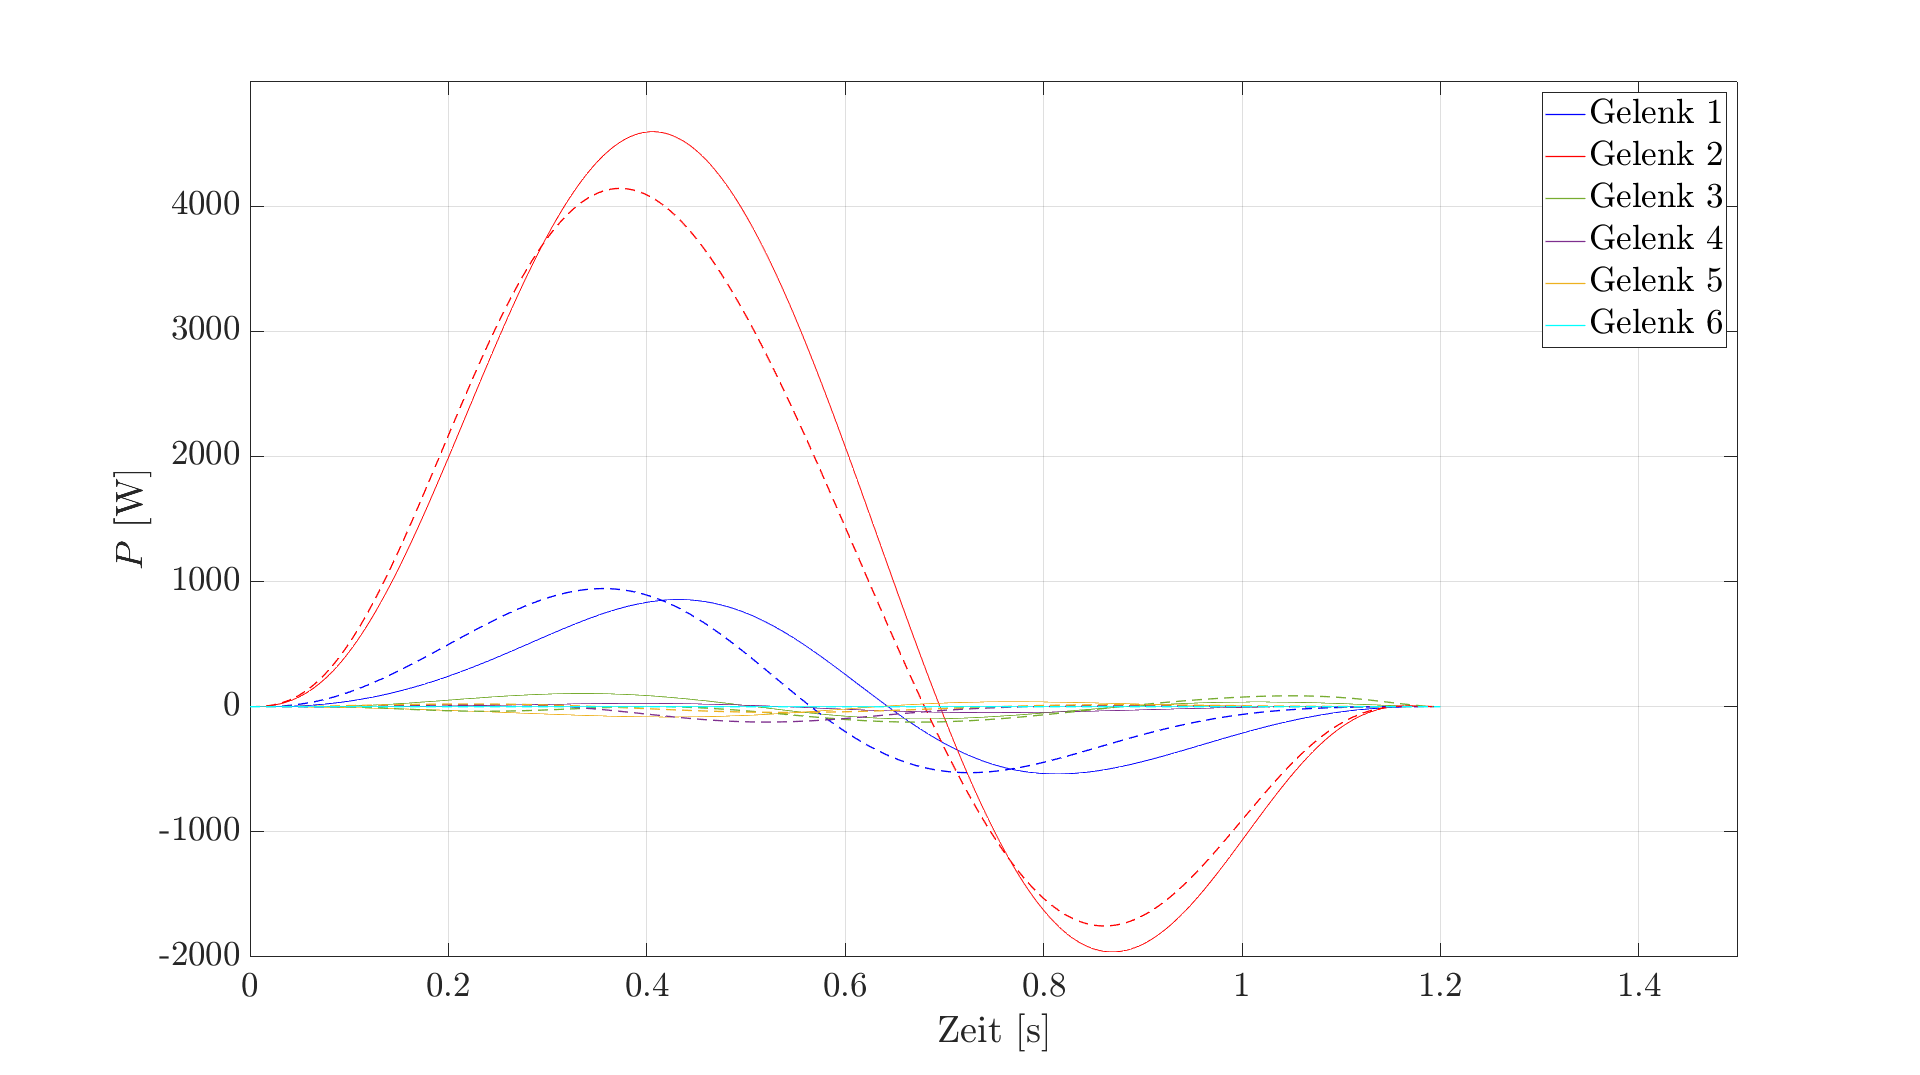
\includegraphics[width=1\linewidth]{images/Optimierungsergebnisse_up/popt}
	\caption{Simulierte Leistungsaufnahme der Initialbahn und optimierten Bewegungsbahn}
	\label{fig:popt}
\end{figure}
%
Nachfolgend werden die Geschwindigkeitsnebenbedingungen in Abbildung \ref{fig:velopt} sowie der Verlauf der Gelenkwinkel in Abbildung \ref{fig:posopt} untersucht. 
%
\begin{figure}[tbph]
	\centering
	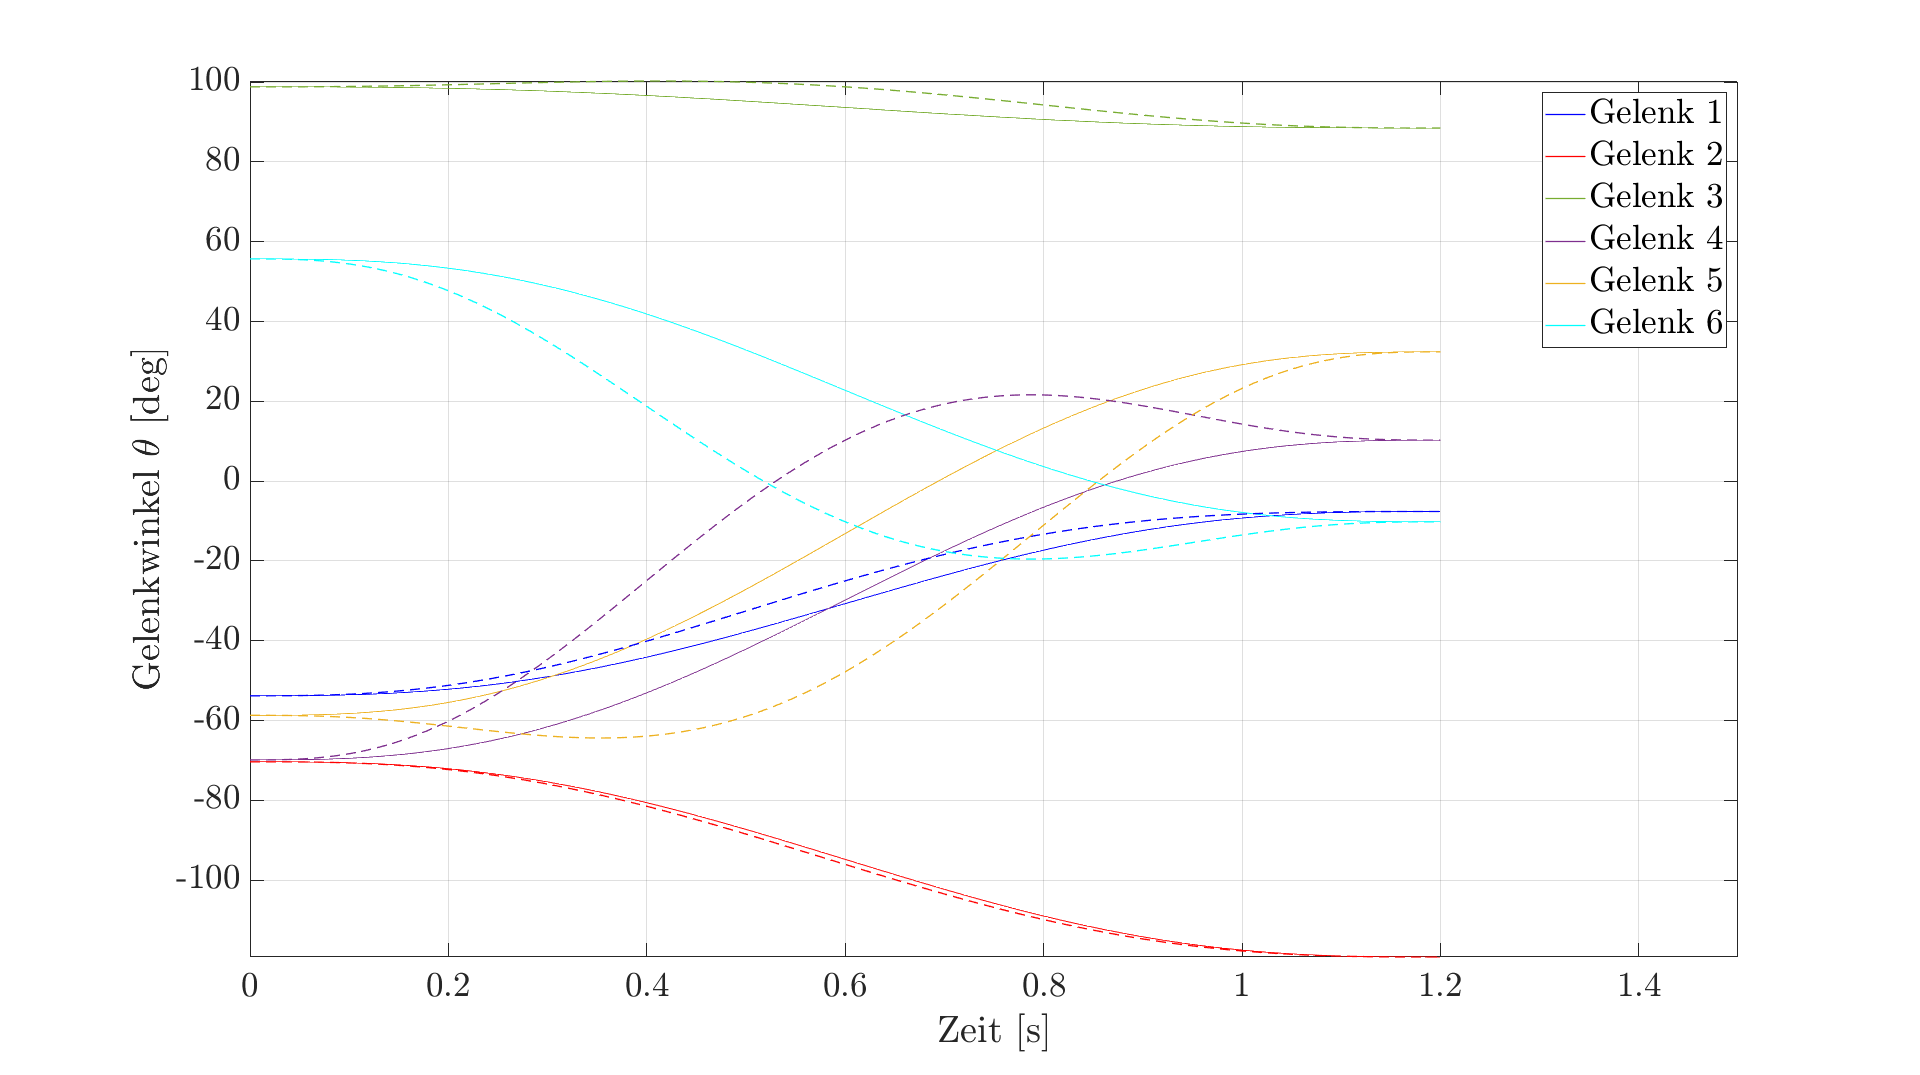
\includegraphics[width=1\linewidth]{images/Optimierungsergebnisse_up/posopt}
	\caption{Gelenkwinkelverläufe der Initialbahn und energieoptimierten Bewegungsbahn}
	\label{fig:posopt}
\end{figure}
%
\begin{figure}[tbph]
	\centering
	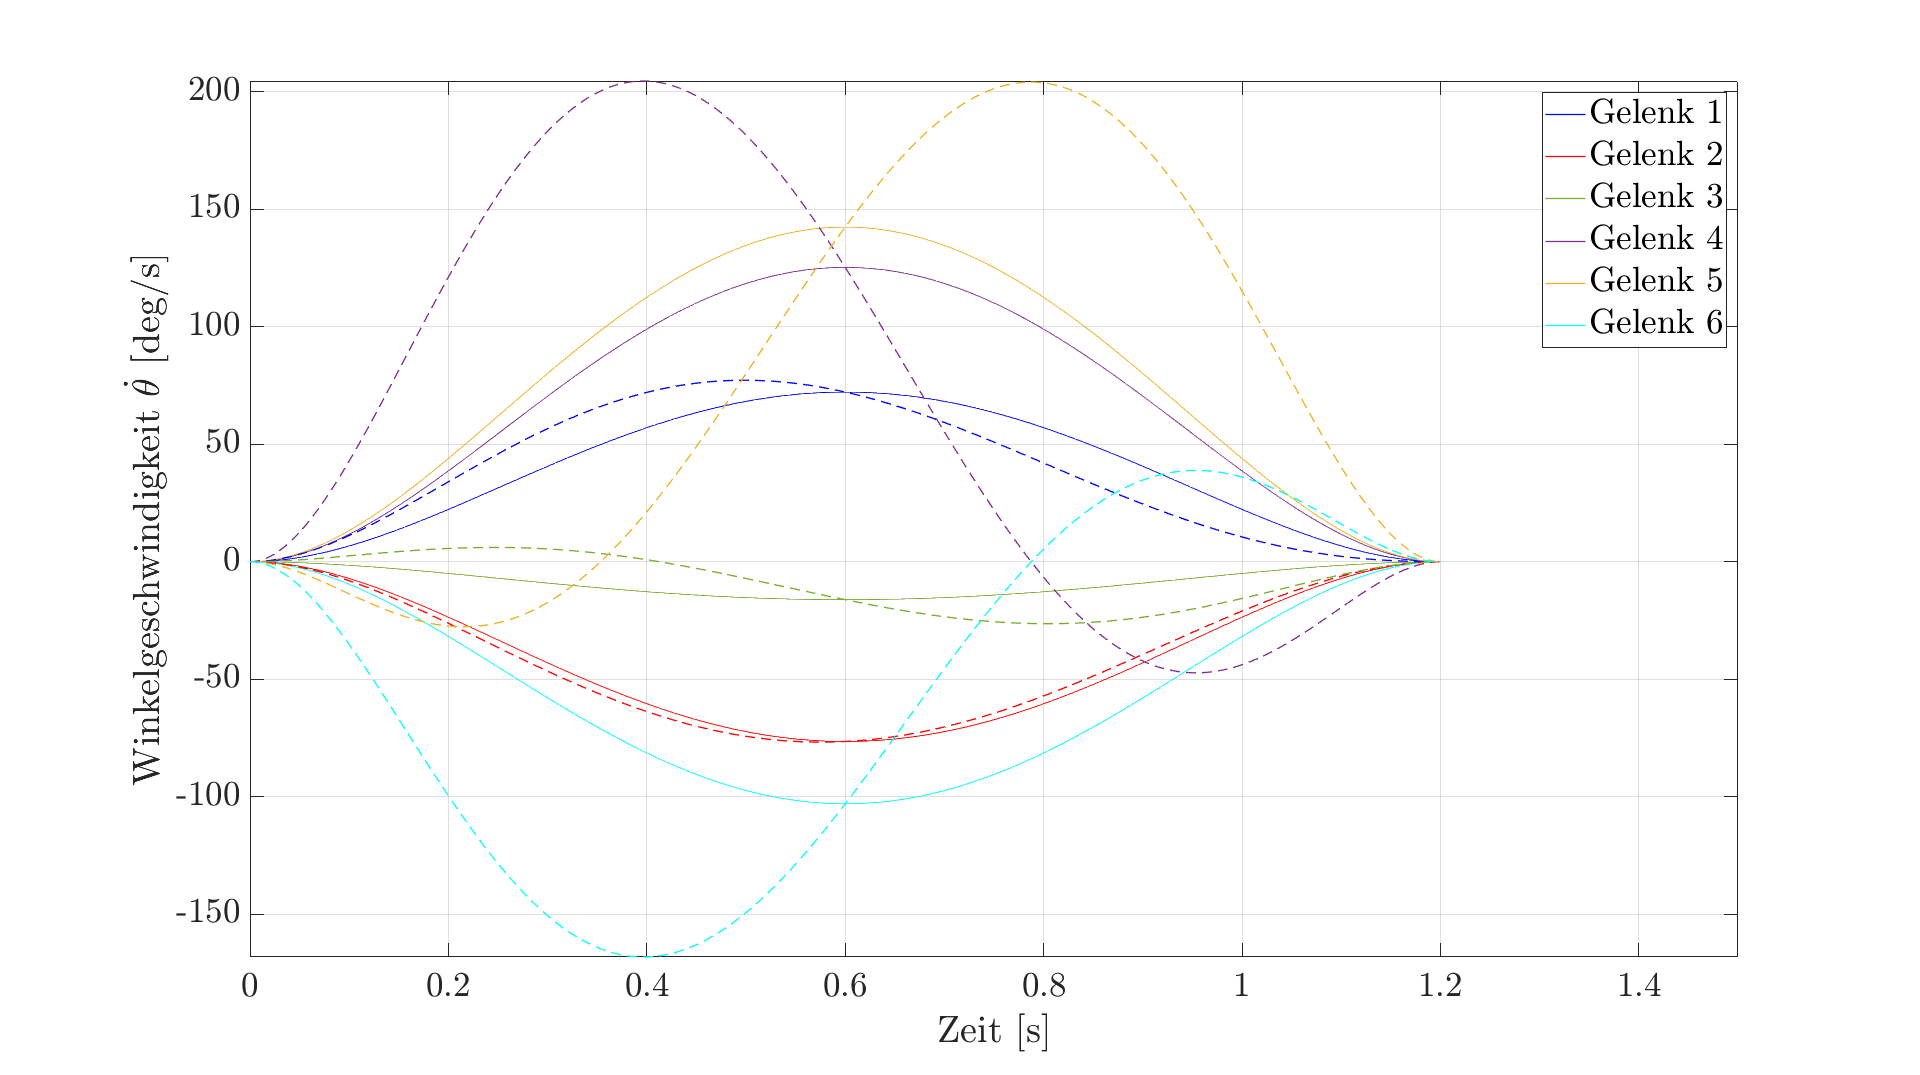
\includegraphics[width=1\linewidth]{images/Optimierungsergebnisse_up/velopt}
	\caption{Winkelgeschwindigkeitsverläufe der Initialbahn und energieoptimierten Bewegungsbahn}
	\label{fig:velopt}
\end{figure}
%
Für den Verlauf der Winkel im zweiten Gelenk sind keine auffälligen Abweichungen von der Initialbahn zu erkennen. Die beiden Verläufe der Gelenkwinkel eins und drei zeigen geringe Abweichungen im Bereich der Via-Punkte. Signifikante Unterschiede sind für die Verläufe der Gelenkwinkel vier, fünf und sechs erkennbar.  Bei Betrachtung der Abbildung \ref{fig:velopt} fällt auf, dass die Winkelgeschwindigkeiten $\dot{q}_{4}(t)$, $\dot{q}_{5}(t)$ und $\dot{q}_{6}(t)$ erheblich größer ausfallen als die Originalverläufe. Dies ist auf die Nähe der Gelenkwinkel ${q}_{v,4}$, ${q}_{v,5}$ und ${q}_{v,6}$ zu den Grenzwerten in Kombination mit der Größe des Gelenkwinkelhub $\Delta q_i = | q_{s,i}+q_{e,i} | ~\forall~ i \in \{4,5,6\}$ zurückzuführen. Infolgedessen werden die Via-Punkte ${q}_{v,4}$, ${q}_{v,5}$ und ${q}_{v,6}$ manuell auf den Mittelwert zwischen Initial-Via-Punkt und energie-optimalen Via-Punkt, siehe Gleichung \ref{eqn:manuellejustage} nachjustiert.
%
\begin{equation}
	\label{eqn:manuellejustage}
	{q}_{v,i,justiert} = \dfrac{{q}_{v,i,opt} + \dfrac{q_{s,i}+q_{e,i}}{2}}{2}~\forall~ i \in \{4,5,6\}
\end{equation}
%
Die resultierenden Winkelgeschwindigkeiten in Abbildung \ref{fig:veloptedit} und Winkelbeschleunigungen in Abbildung \ref{fig:accoptedit}  werden damit auf ein akzeptables Maß reduziert. Die energie-optimalen Verläufe sind gestrichelt, die justierten Verläufe gepunktet dargestellt.
%
\begin{figure}[tbph]
	\centering
	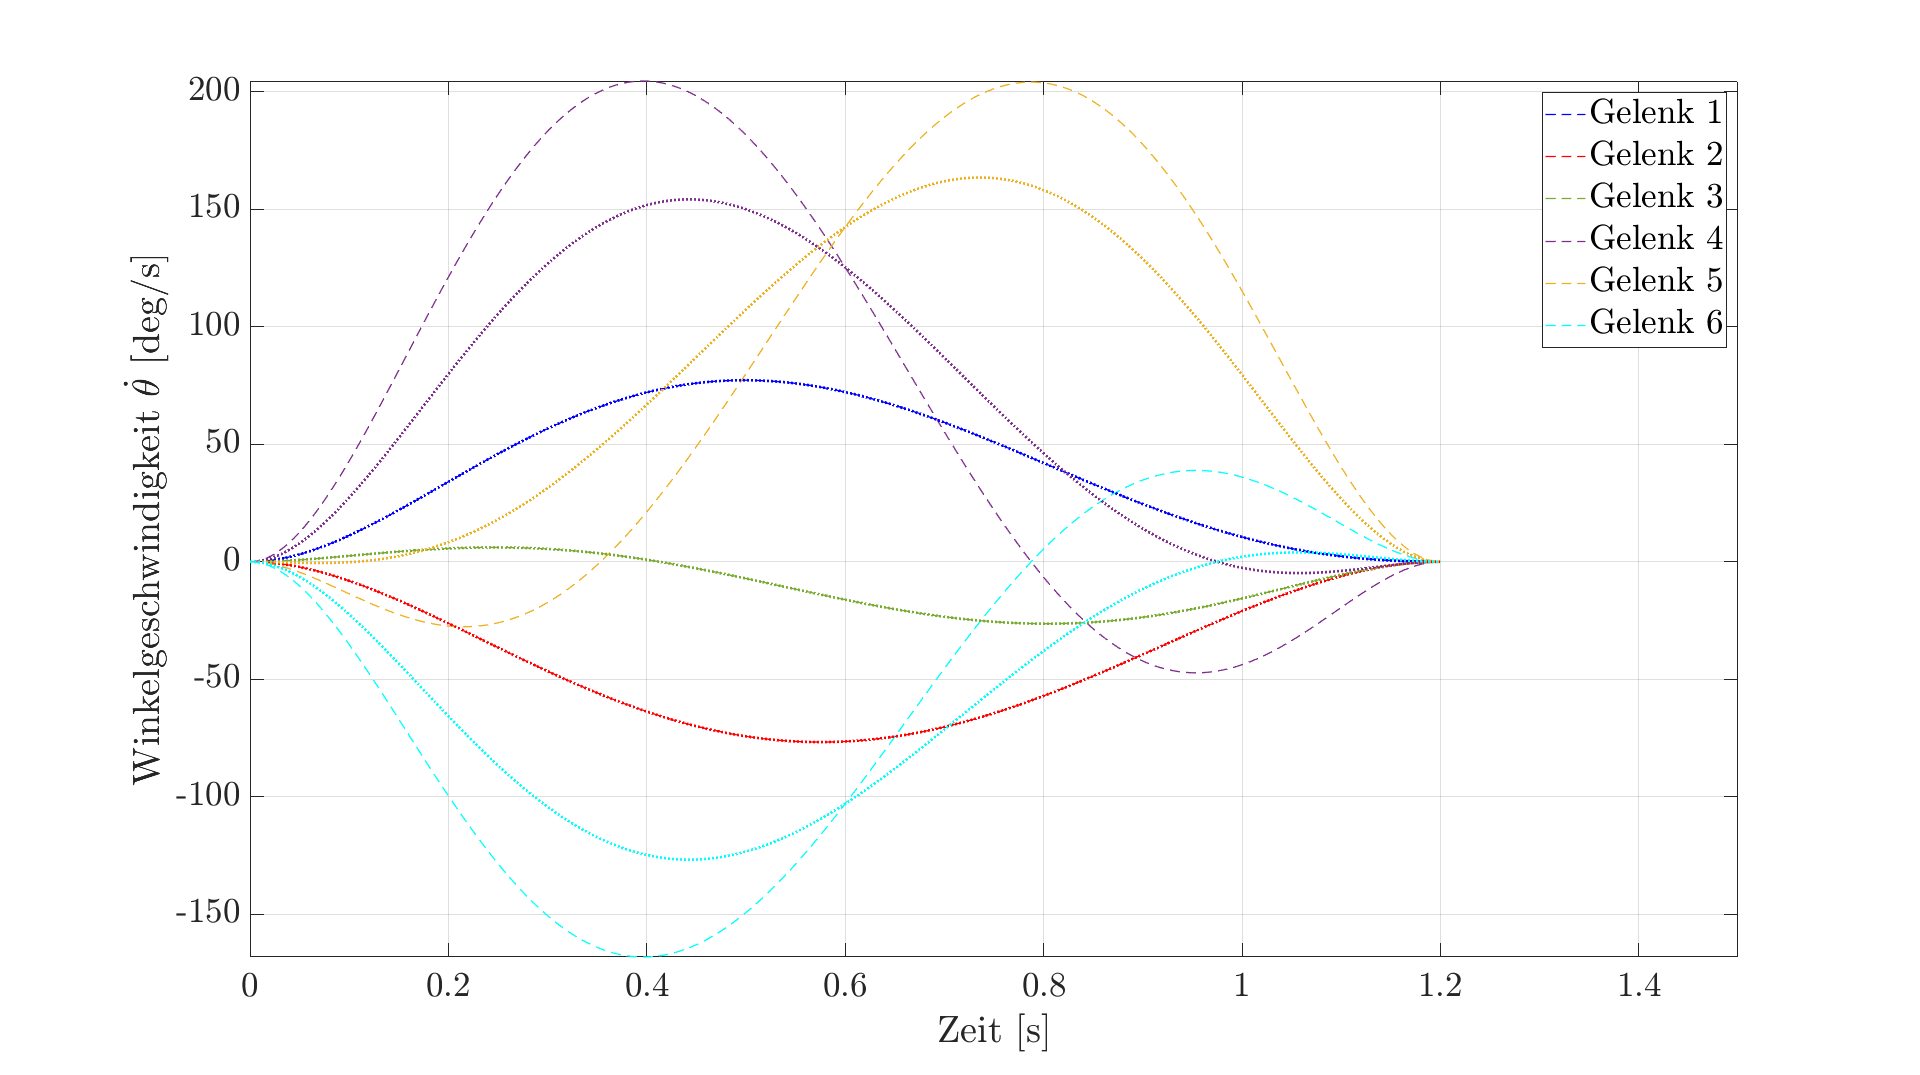
\includegraphics[width=1\linewidth]{images/Optimierungsergebnisse_up/veloptedit}
	\caption{Winkelgeschwindigkeitsverläufe der energieoptimierten Bewegungsbahn und justierten energieoptimierten Bewegungsbahn}
	\label{fig:veloptedit}
\end{figure}
%
\begin{figure}[tbph]
	\centering
	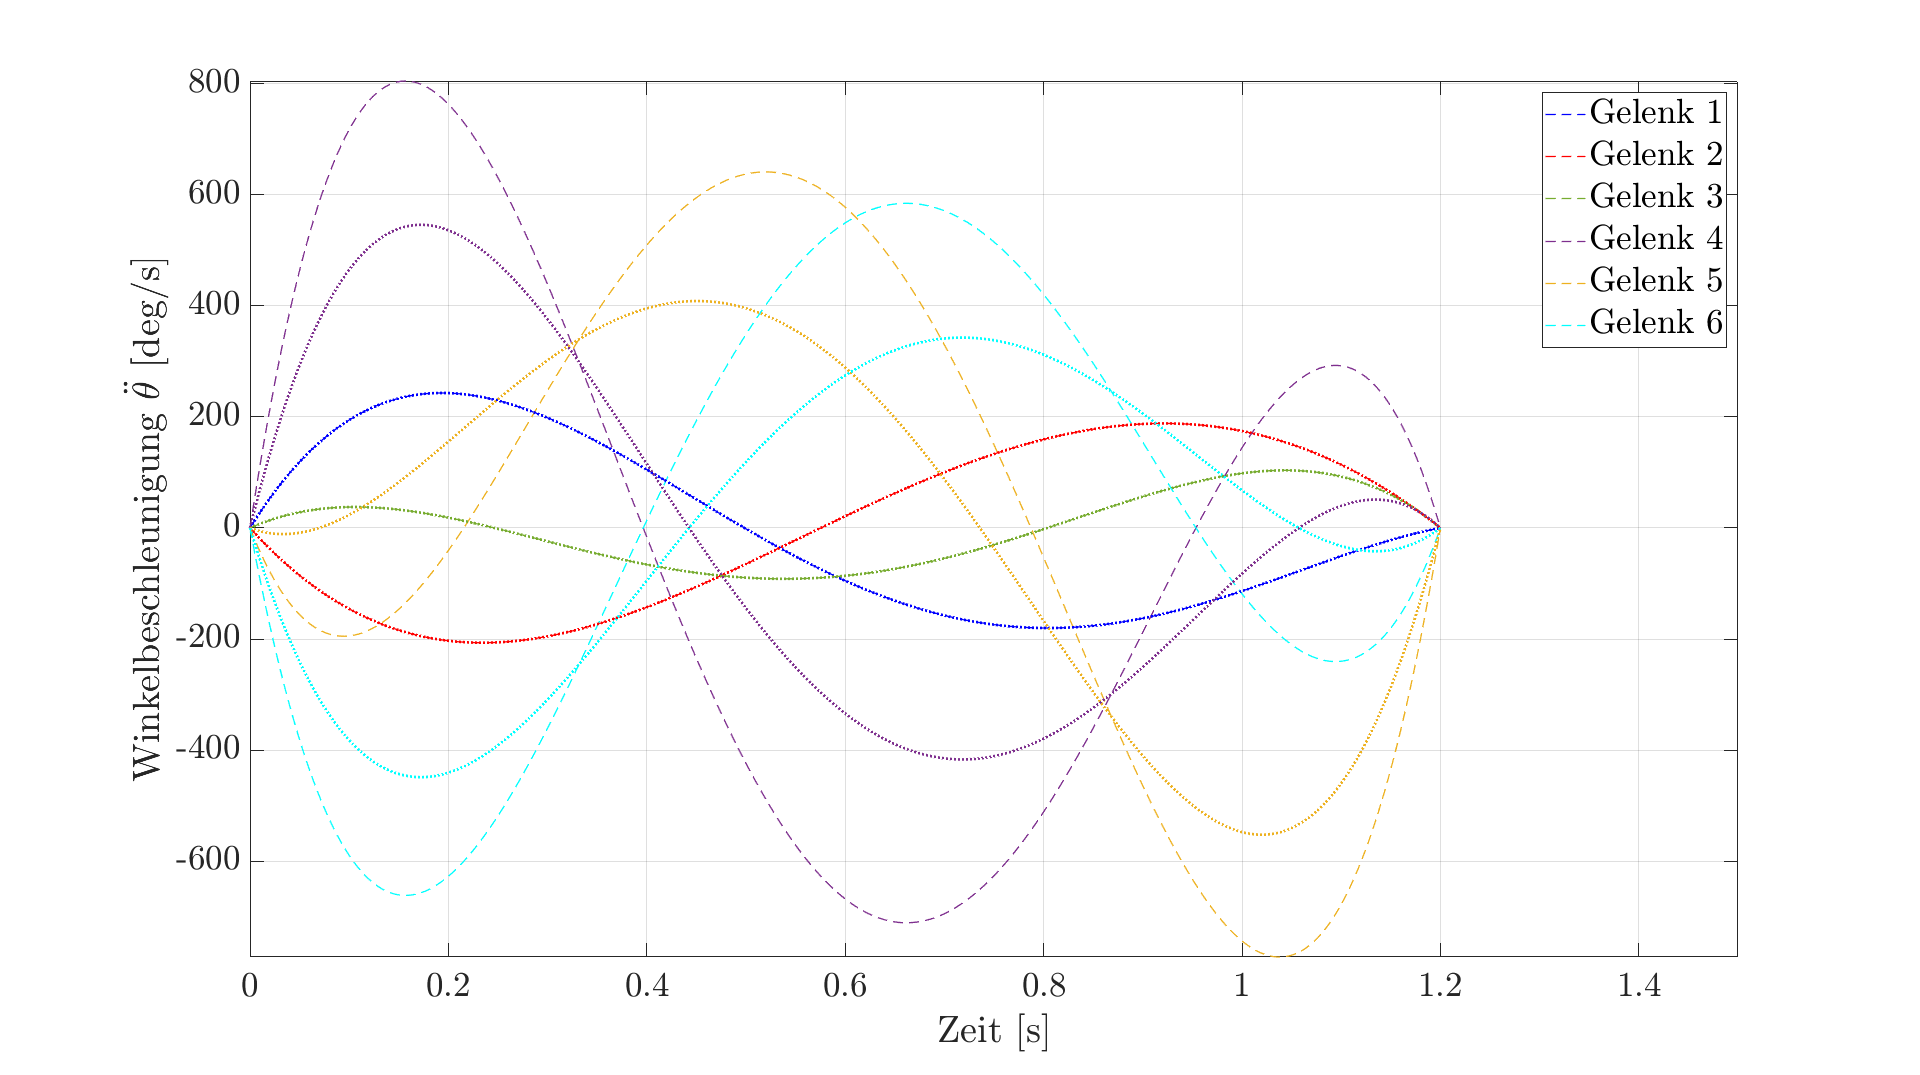
\includegraphics[width=1\linewidth]{images/Optimierungsergebnisse_up/accoptedit}
	\caption{Winkelbeschleunigungsverläufe der energieoptimierten Bewegungsbahn und justierten energieoptimierten Bewegungsbahn}
	\label{fig:accoptedit}
\end{figure}
%
Für den justierten Parametervektor beträgt der Energieverbrauch 1858 Joule. Damit wird eine Energieeinsparung von 7,15 \% gegenüber der Initialbahn erzielt. Die Abbildungen für den Vergleich der initialen und justierten Verläufe aller relevanten Größen sind im Anhang \ref{acc:optupjust} aufgeführt.
%
\section{Validierung der Optimierungsergebnisse}
Im Rahmen der Validierung werden die Simulationsergebnisse der Energieeinsparung am realen System überprüft. Dazu wird der 
justierte-energieoptimierte Via-Punkts \lstinline{ViaJustOptUp}
im Programm $Kleben-Seitenwand$ auf der KR C5 angelegt. In der Standarddefinition des Via-Punkts fährt der Roboter diesen millimetergenau an. Hierbei reduziert er seine Geschwindigkeit bei Erreichen des Punkts auf Null. 
%
\begin{lstlisting}[numbers=none]
	;FOLD PTP ViaJustOptUp Vel=100 % PDAT8 Tool[1] Base[0] ;%{PE}
\end{lstlisting}
%
Ziel der Optimierung ist nicht die Anpassung des zeitlichen Verhaltens. Eine signifikante Abweichung von der originalen Bewegungsdauer ist deshalb unzulässig. Im Rahmen der Implementierung des Via-Punkts auf der KR C5 wird dieser um einen \lstinline{CONT} 
Überschleifbefehl erweitert. 
%
\begin{lstlisting}[numbers=none]
	;FOLD PTP ViaJustOptUp CONT Vel=100 % PDAT8 Tool[1] Base[0] ;%{PE}
\end{lstlisting}
%
In der Parameterdefinition \lstinline{PDAT} 
wird der Modus der Approximation \lstinline{APO_MODE}  
des Via-Punkts \lstinline{ViaJustOptUp}
mit \lstinline{CDIS}  
festgelegt. D. h. ein Überschleifen beginnt frühestens, wenn die Entfernung zum Punkt den Wert von \lstinline{APO_DIST}    
unterschreitet \cite[S.~578]{KSS.2023}.
%
\begin{lstlisting}[numbers=none]
	DECL PDAT PPDAT8={VEL 100.0000,ACC 100.000,APO_DIST 500.000,APO_MODE #CDIS,GEAR_JERK 100.000,EXAX_IGN 0}
\end{lstlisting}
Die maximale Überschleifdistanz wird auf 500 mm definiert. Von einem vollen Überschliff mit 1000 mm wird Abstand genommen, um das Risiko einer Kollision des Roboters mit peripheren Bauteilen nicht zu maximieren. Die Bewegung vom Startpunkt über den Via-Punkt zum Zielpunkt wird zunächst auf Kollisionsfreiheit durch manuelles Abfahren mit reduzierter Geschwindigkeit in der KUKA Betriebsart T1 getestet. Nach einer Verifizierung der Überschleif-Bewegung für eine programmierte Geschwindigkeit von 50\% in der Betriebsart T2 erfolgt die Signalaufzeichnung der justierten-energieoptimierten Trajektorie mit eine programmierten Geschwindigkeit von 100\%. Die über alle sechs Gelenke summierte Leistungsaufnahme des Roboters  wird in \ref{fig:pup} abgebildet. 
%
\begin{figure}[tbph]
	\centering
	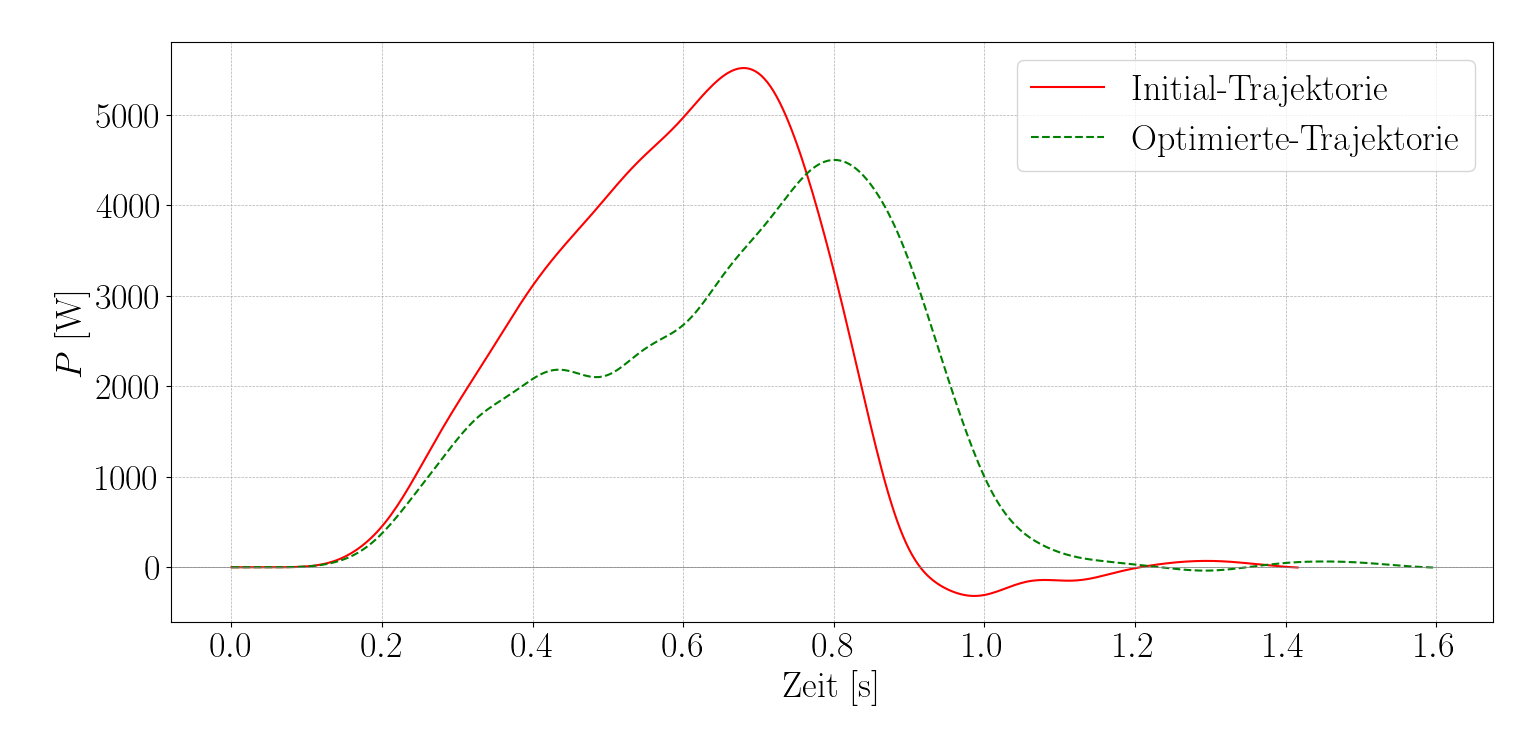
\includegraphics[width=1\linewidth]{images/P_up}
	\caption{Summierte Leistungsaufnahme des Roboters für den Verfahrweg vom letzten Prozesspunkt auf die  Home Position im Programm $Kleben-Seitenwand$}
	\label{fig:pup}
\end{figure}
%
Dabei ist die Bewegungsdauer der justierten-energieoptimierten Trajektorie ca. 0,2 s länger als die der Initial-Trajektorie. In der PTP-Bewegungsart führt der Roboter den Tool-Center-Point (TCP) entlang der schnellsten Bahn zum Zielpunkt \cite[S.~429]{KSS.2023}. Die Zunahme wird der Definition des Via-Punkts mit \lstinline{CDIS=500 mm}
zugeschrieben. Da dieser zusätzlich in der Bahnplanung berücksichtigt wird, bewegt sich der TCP nicht mehr auf der schnellsten Bahn. Die erzielte Energieeinsparung wird in \ref{fig:eup500} gezeigt. Dabei wird die Prognose der Simulation erfüllt, dass die höchste Einsparung für das zweite Gelenk erreicht wird. Wie erwartet ist für den mechanischen Energieverbrauch im ersten Gelenk eine leichte Zunahme festzustellen.  Die Optimierungsergebnisse werden anhand des qualitativen Verlaufs als plausibel eingestuft. Für einen quantitativen Vergleich sind die Tabellen \ref{tab:energieverbrauch-simuliert} und \ref{tab:energieverbrauch-gemessen} heranzuziehen. Dass der gemessene Energieverbrauch ca. 25 \% höher ausfällt wird darauf zurückgeführt, dass das Modell den Verbrauch in den Gelenken drei bis sechs signifikant geringer berechnet. Die gemessene Einsparung fällt mit 11,7 \% höher aus als in der Simulation. Dabei ist die Zunahme der Bewegungsdauer zu berücksichtigen. 
%
\begin{figure}[tbph]
	\centering
	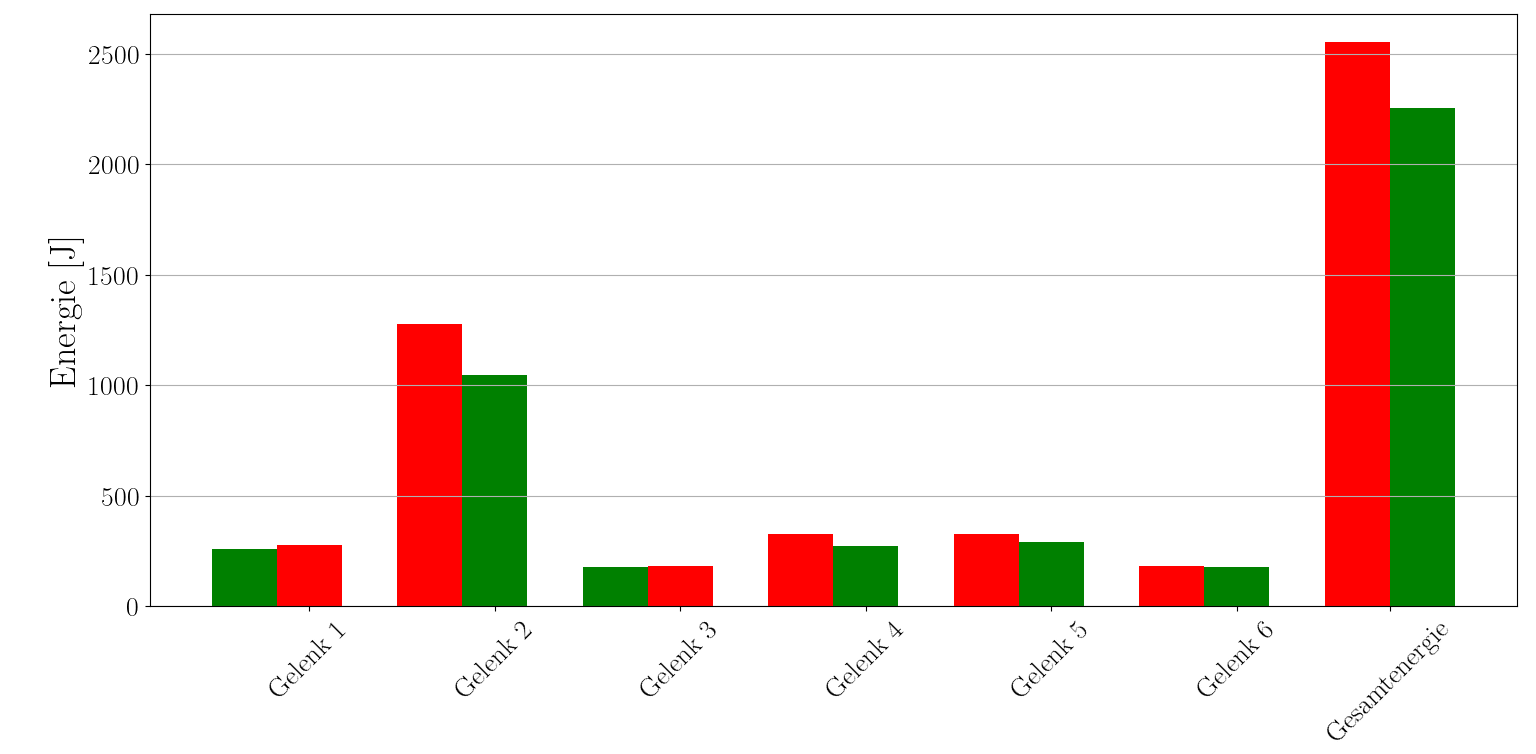
\includegraphics[width=1\linewidth]{images/e_up500}
	\caption{Energieverbrauch des Roboters für den Verfahrweg vom letzten Prozesspunkt auf die  Home Position im Programm $Kleben-Seitenwand$}
	\label{fig:eup500}        
\end{figure}
%
\begin{table}[tbph]
	\centering
	\caption{Energieverbrauch simuliert $Kleben-Seitenwand$ Verfahrweg vom letzten Prozesspunkt auf die  Home Position}
	\label{tab:energieverbrauch-simuliert}
	\begin{tabular}{|c|c|c|c|}
		\hline
		Trajektorie & Größe & Einheit & Wert \\
		\hline
		Initial & Energieverbrauch & [kJ] &2.001  \\
		\hline
		Justiert-Energieoptimiert & Energieverbrauch & [kJ] &1.858  \\
		\hline
		& Energieeinsparung & [kJ] &0.143  \\
		\hline
		& Energieeinsparung & [\%] &7,15  \\
		\hline
	\end{tabular}
	\centering
	\caption{Energieverbrauch gemessen $Kleben-Seitenwand$ Verfahrweg vom letzten Prozesspunkt auf die  Home Position}
	\label{tab:energieverbrauch-gemessen}
	\begin{tabular}{|c|c|c|c|}
		\hline
		Trajektorie & Größe & Einheit & Wert \\
		\hline
		Initial & Energieverbrauch & [kJ] &2.553  \\
		\hline
		Justiert-Energieoptimiert & Energieverbrauch & [kJ] &2.254 \\
		\hline
		& Energieeinsparung & [kJ] &0.299  \\
		\hline
		& Energieeinsparung & [\%] &11,7 \\
		\hline
	\end{tabular}
\end{table}
%\begin{figure}[tbph]
%	\centering
%	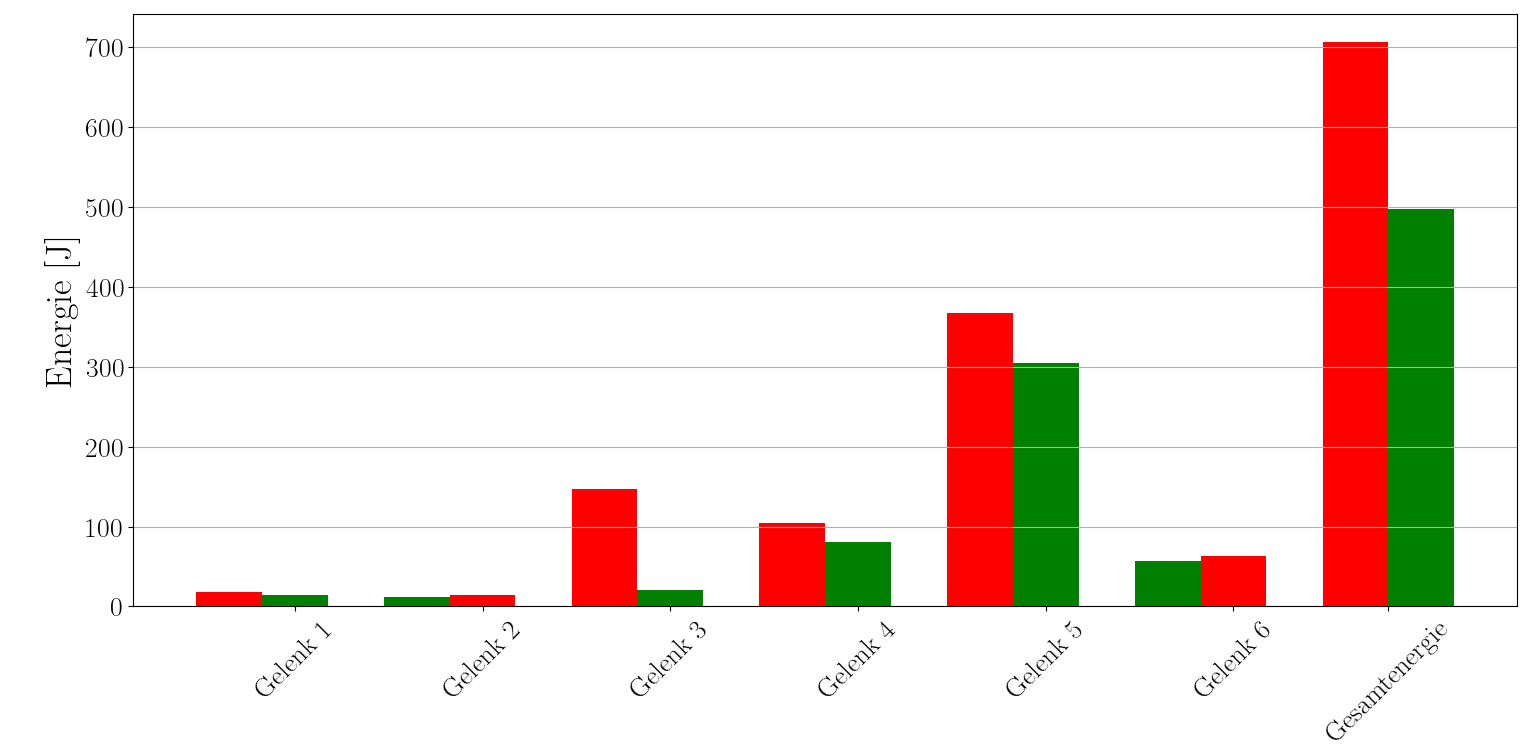
\includegraphics[width=1\linewidth]{images/e_down500}
%	\caption{Energieverbrauch Bewegung Eins}
%	\label{fig:edown500}
%\end{figure}
%\begin{figure}[tbph]
%	\centering
%	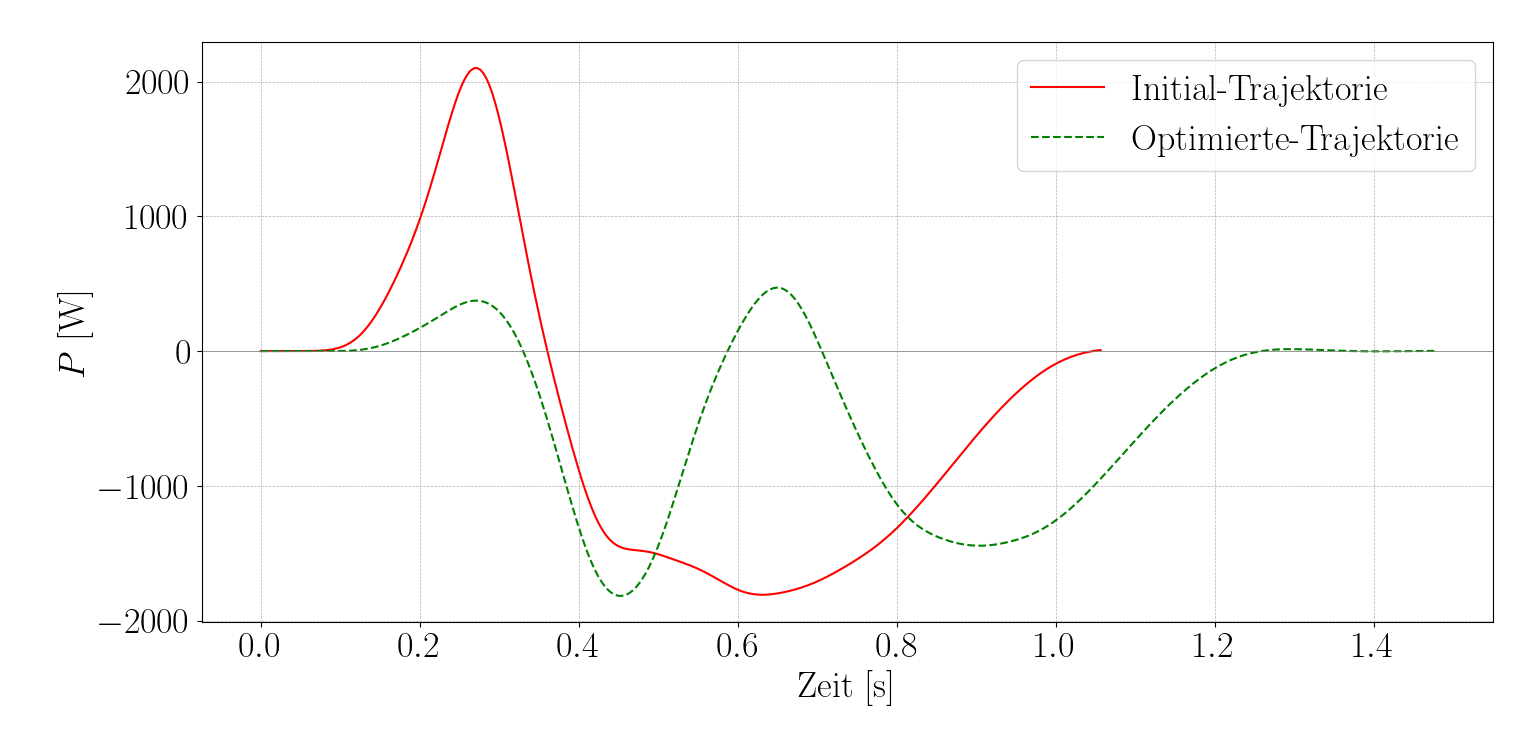
\includegraphics[width=1\linewidth]{images/P_down}
%	\caption{Leistungsaufnahme Bewegung Eins}
%	\label{fig:pdown}
%\end{figure}
%\begin{figure}[tbph]
%	\centering
%	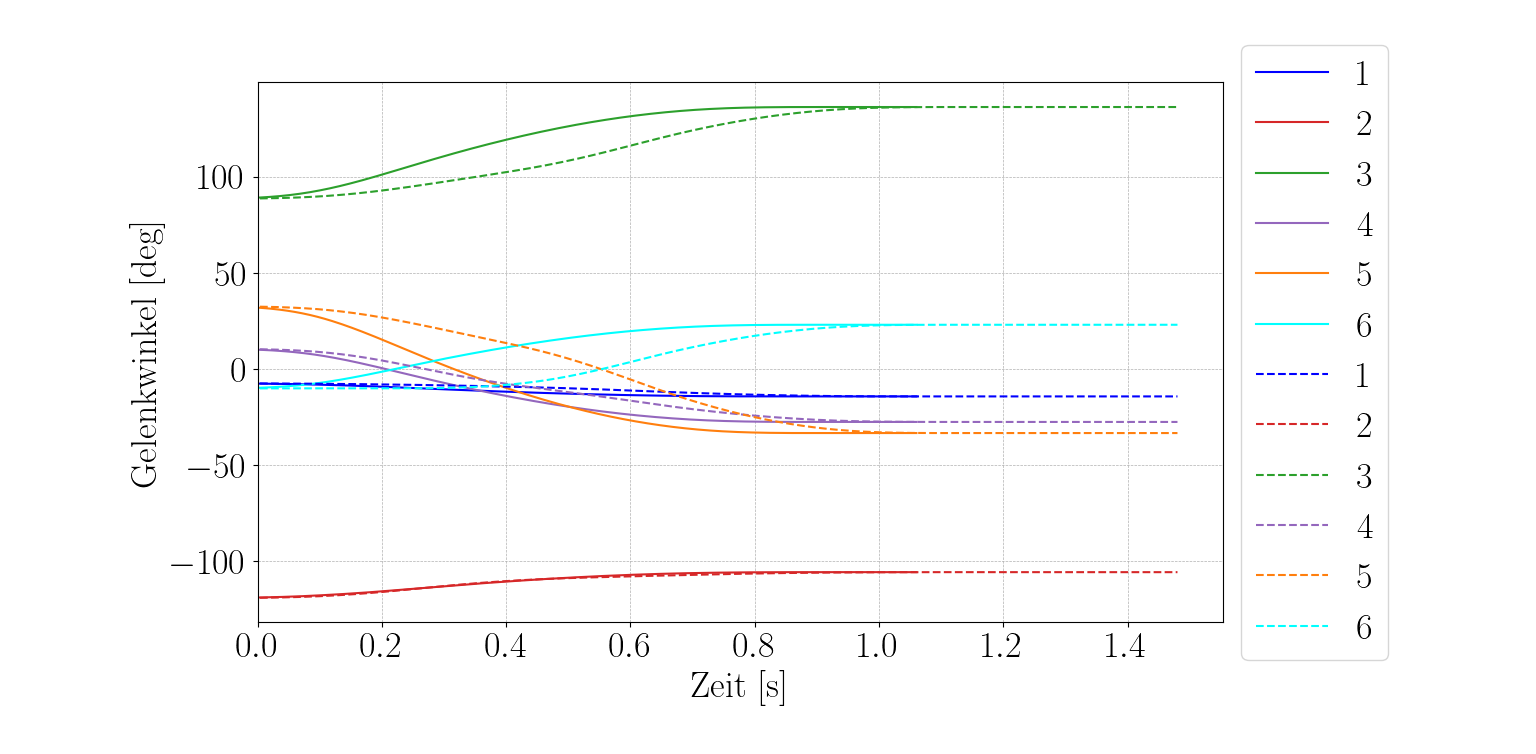
\includegraphics[width=1\linewidth]{images/aiposdown}
%	\caption{Gelenkwinkel Bewegung Eins}
%	\label{fig:aiposdown}
%\end{figure}
%\begin{figure}[tbph]
%	\centering
%	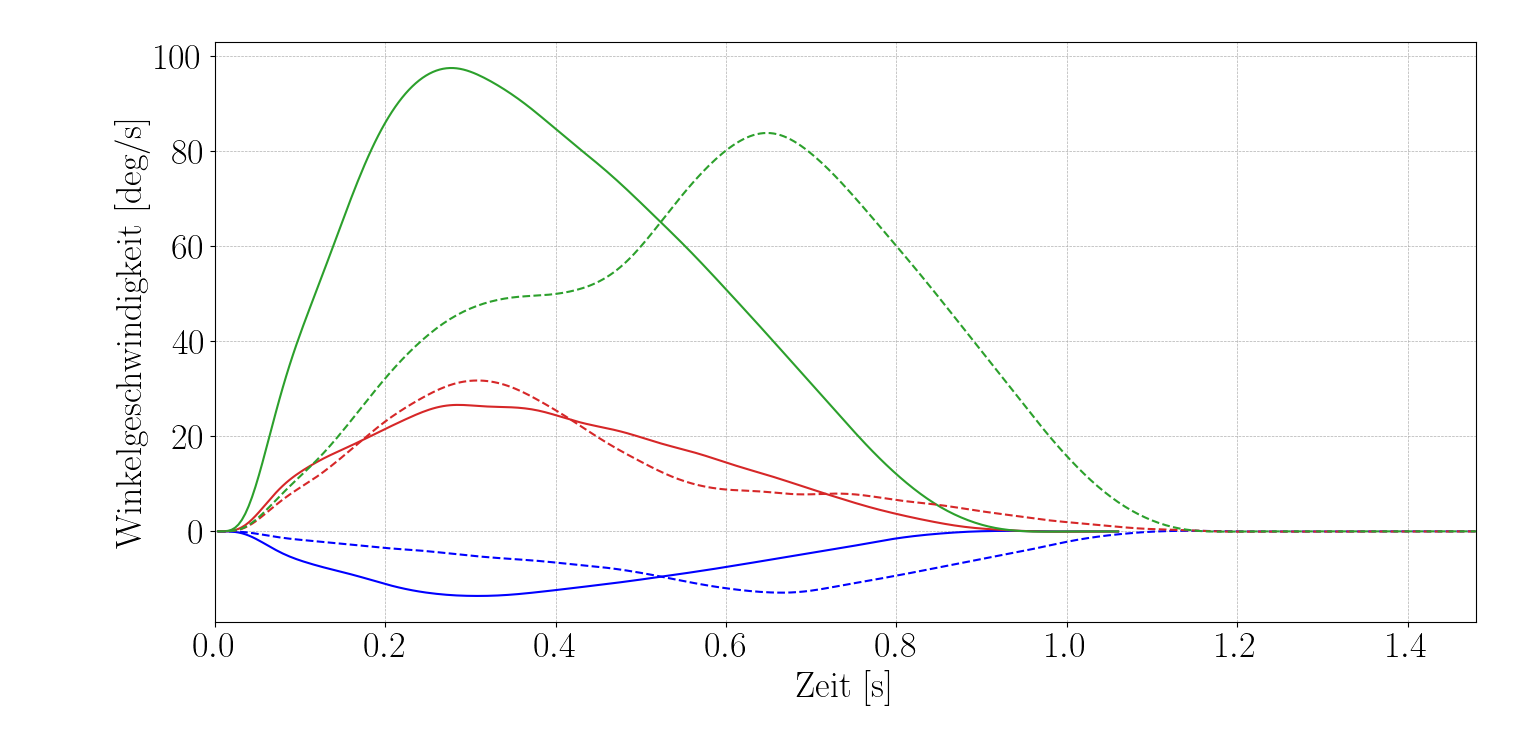
\includegraphics[width=1\linewidth]{images/velposdown1}
%	\caption{Winkelgeschwindigkeit in den Gelenken 1-3 Bewegung Eins}
%	\label{fig:velposdown1}
%\end{figure}
%\begin{figure}[tbph]
%	\centering
%	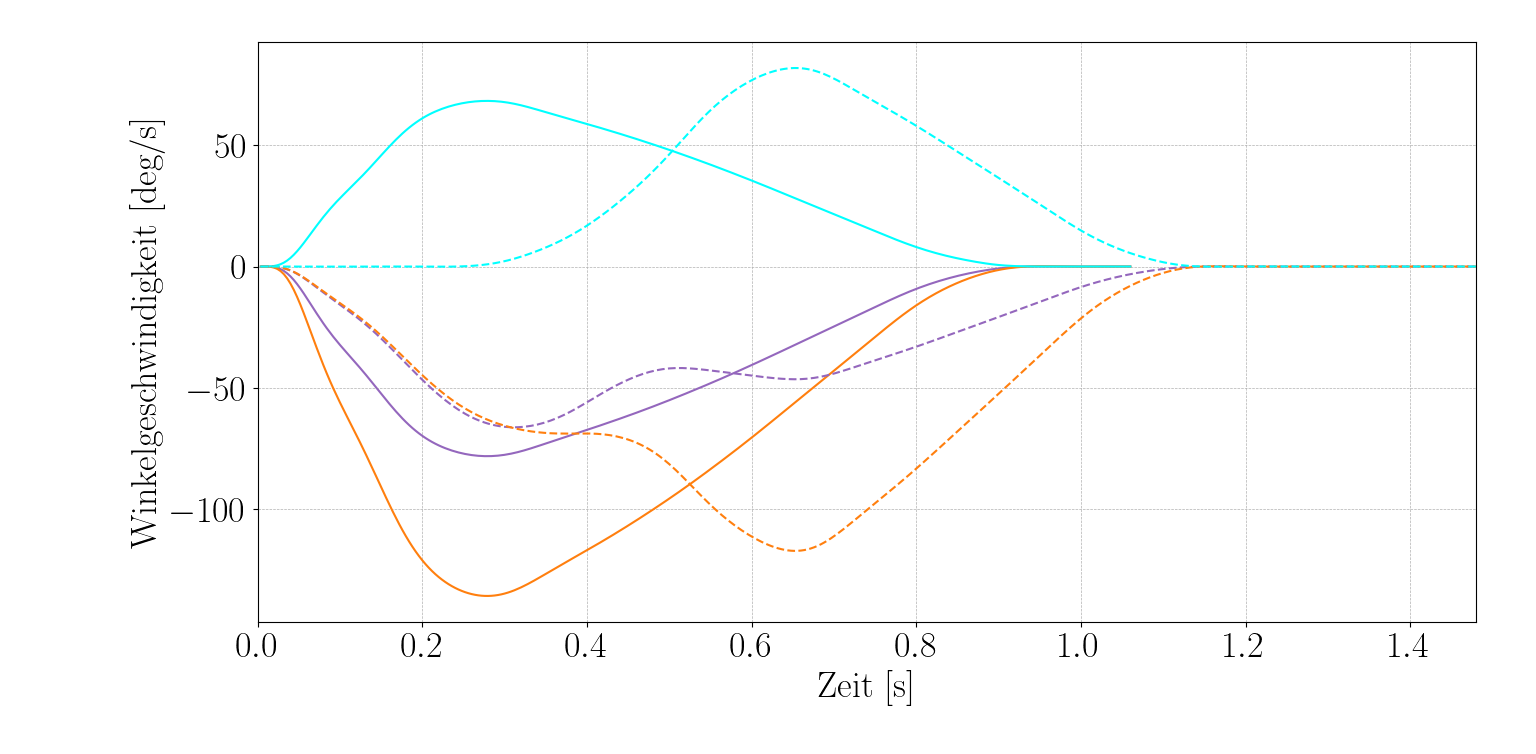
\includegraphics[width=1\linewidth]{images/velposdown2}
%	\caption{Winkelgeschwindigkeit in den Gelenken 4-6 Bewegung Eins}
%	\label{fig:velposdown2}
%\end{figure}
%\begin{figure}[tbph]
%	\centering
%	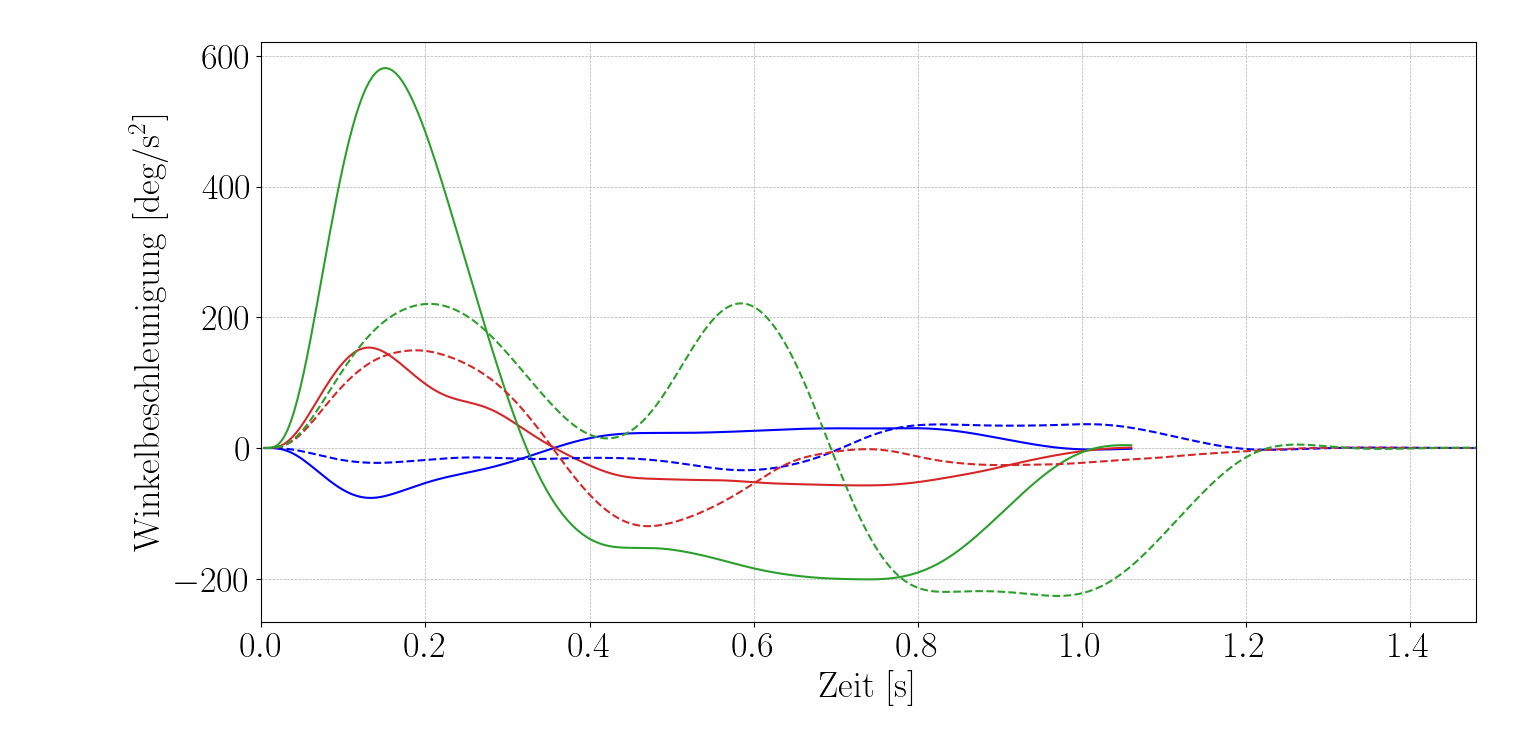
\includegraphics[width=1\linewidth]{images/accdown1}
%	\caption{Winkelbeschleunigung in den Gelenken 1-3 Bewegung Eins}
%	\label{fig:accdown1}
%\end{figure}
%\begin{figure}[tbph]
%	\centering
%	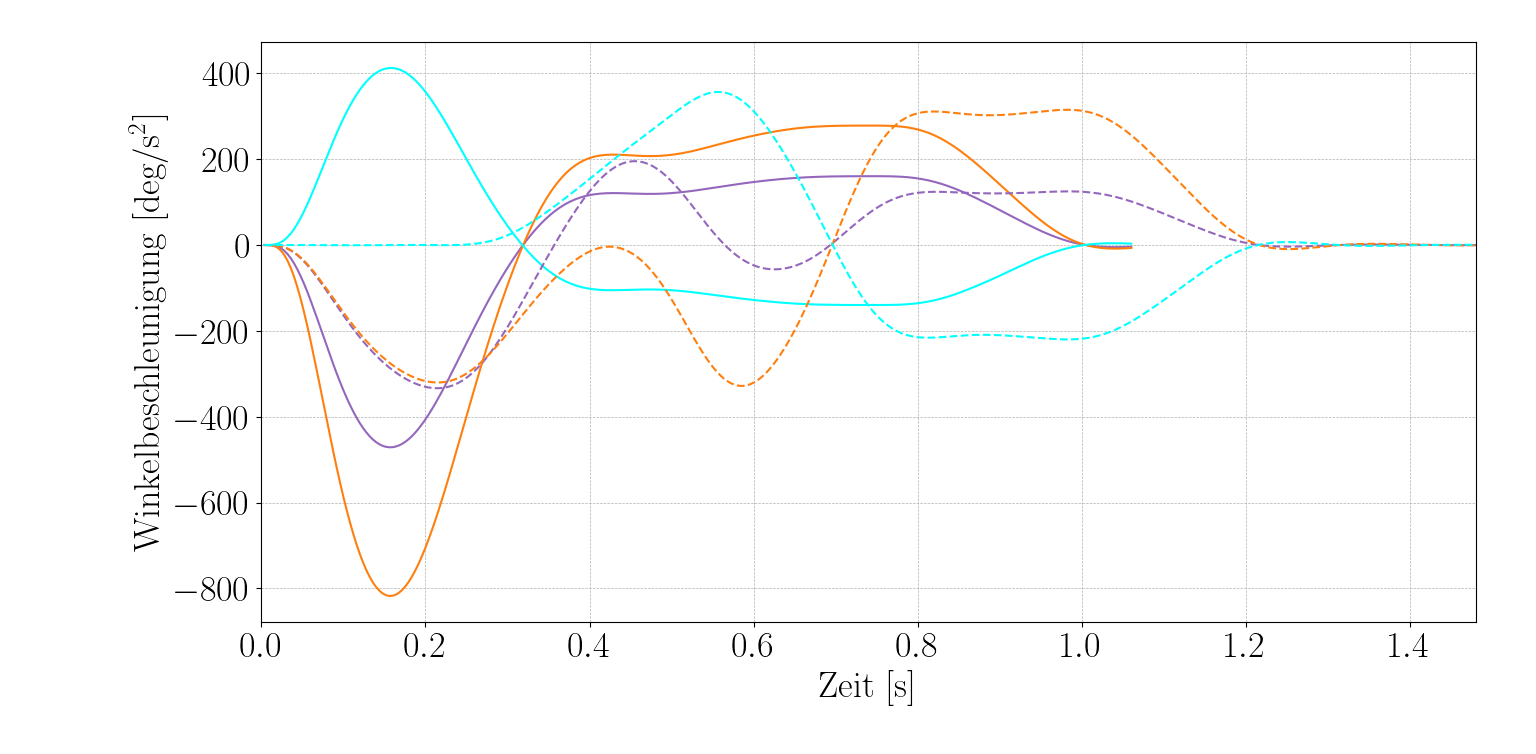
\includegraphics[width=1\linewidth]{images/accdown2}
%	\caption{Winkelbeschleunigung in den Gelenken 4-6 Bewegung Eins}
%	\label{fig:accdown2}
%\end{figure}
%
%\begin{figure}[tbph]
%	\centering
%	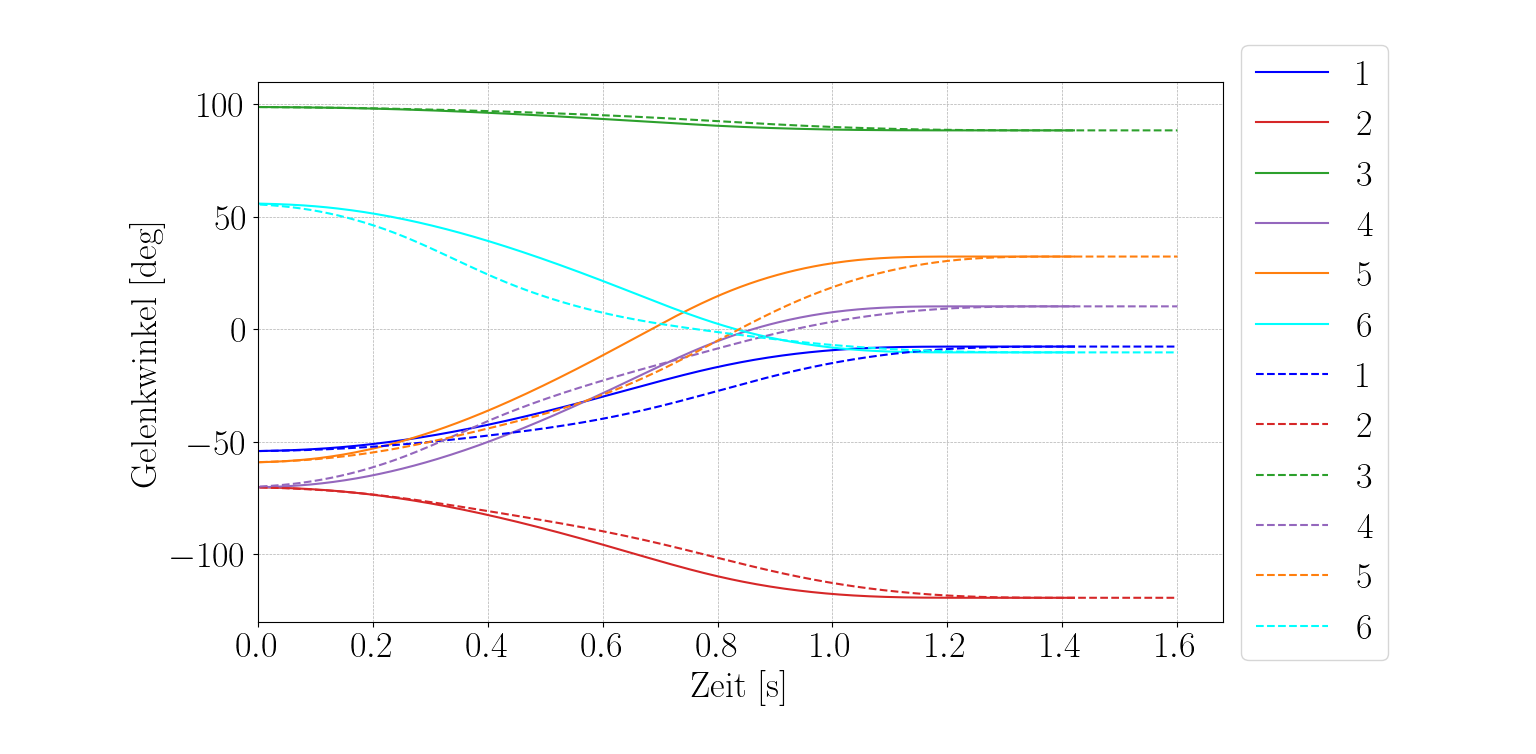
\includegraphics[width=1\linewidth]{images/aiposup}
%	\caption{Gelenkwinkel Bewegung Eins}
%	\label{fig:aiposup}
%\end{figure}
%\begin{figure}[tbph]
%	\centering
%	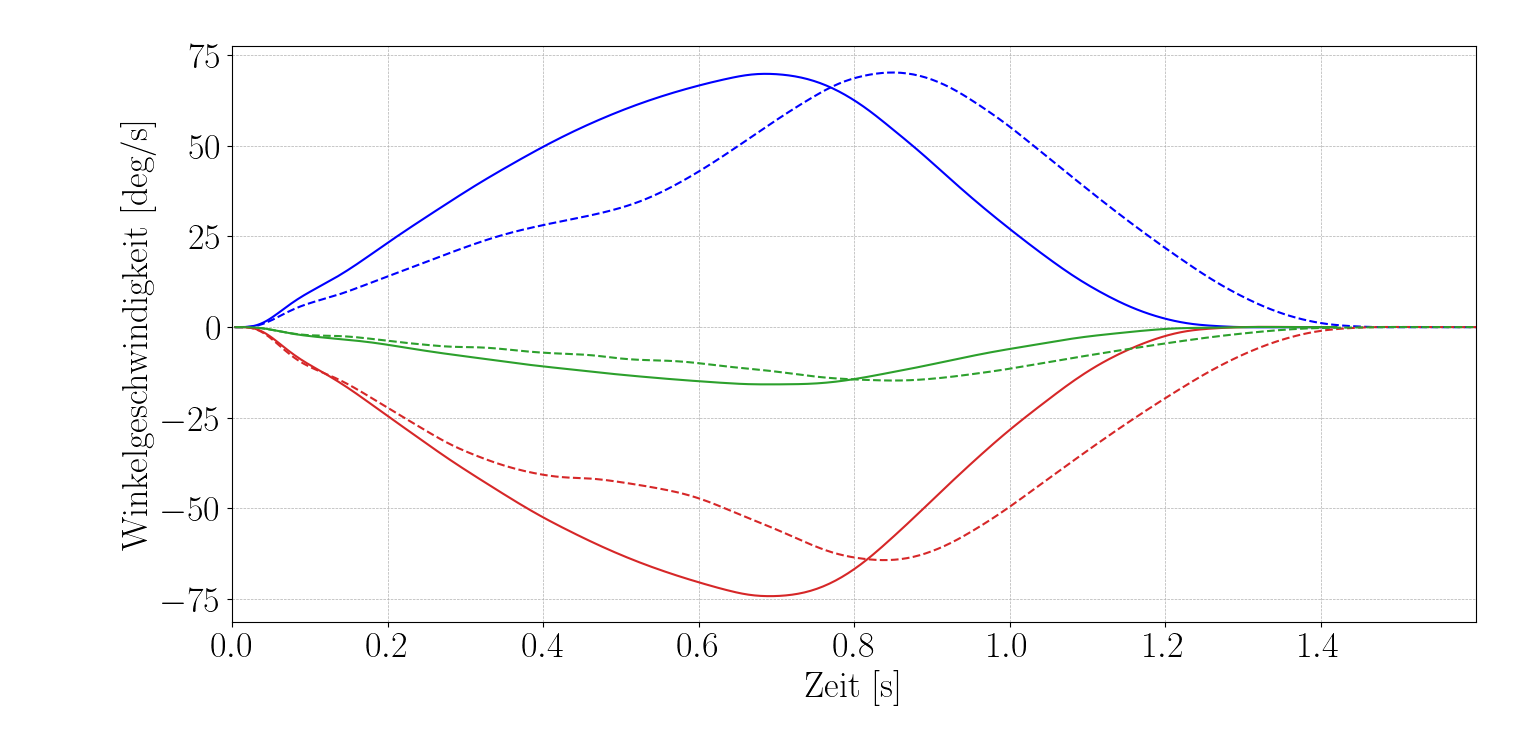
\includegraphics[width=1\linewidth]{images/velposup1}
%	\caption{Winkelgeschwindigkeit in den Gelenken 1-3 Bewegung Zwei}
%	\label{fig:velposup1}
%\end{figure}
%\begin{figure}[tbph]
%	\centering
%	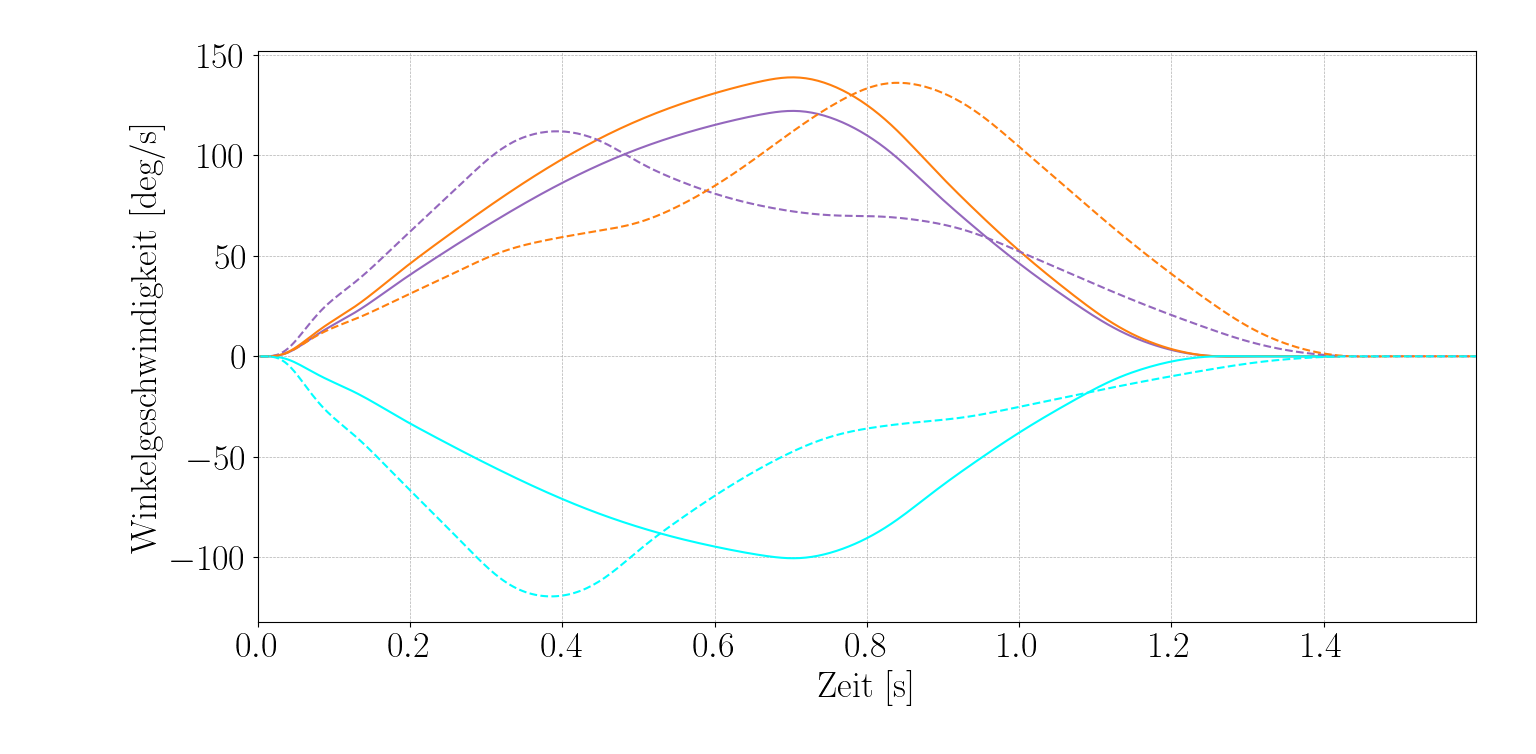
\includegraphics[width=1\linewidth]{images/velposup2}
%	\caption{Winkelgeschwindigkeit in den Gelenken 4-6 Bewegung Zwei}
%	\label{fig:velposup2}
%\end{figure}
%\begin{figure}[tbph]
%	\centering
%	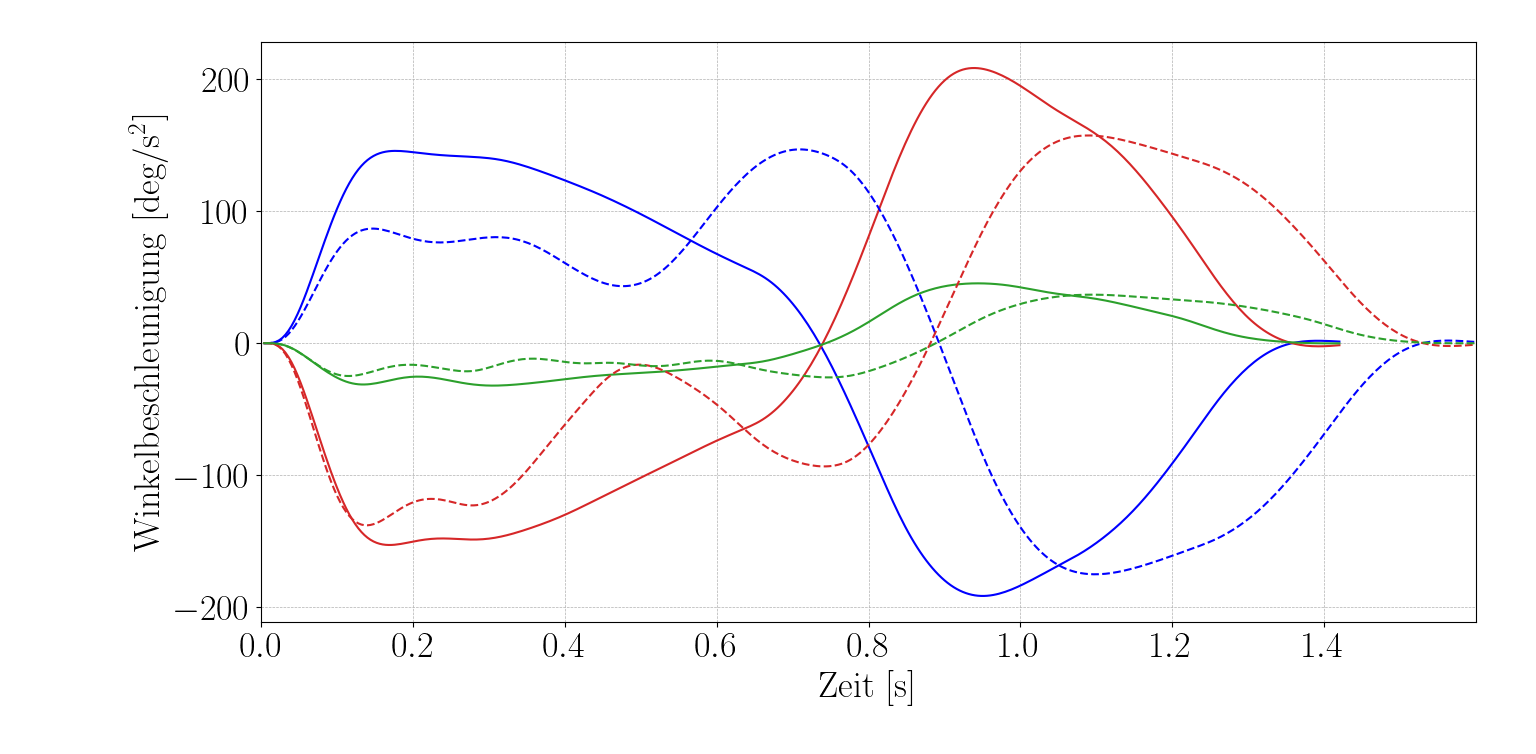
\includegraphics[width=1\linewidth]{images/accup1}
%	\caption{Winkelbeschleunigung in den Gelenken 1-3 Bewegung Zwei}
%	\label{fig:accup1}
%\end{figure}
%\begin{figure}[tbph]
%	\centering
%	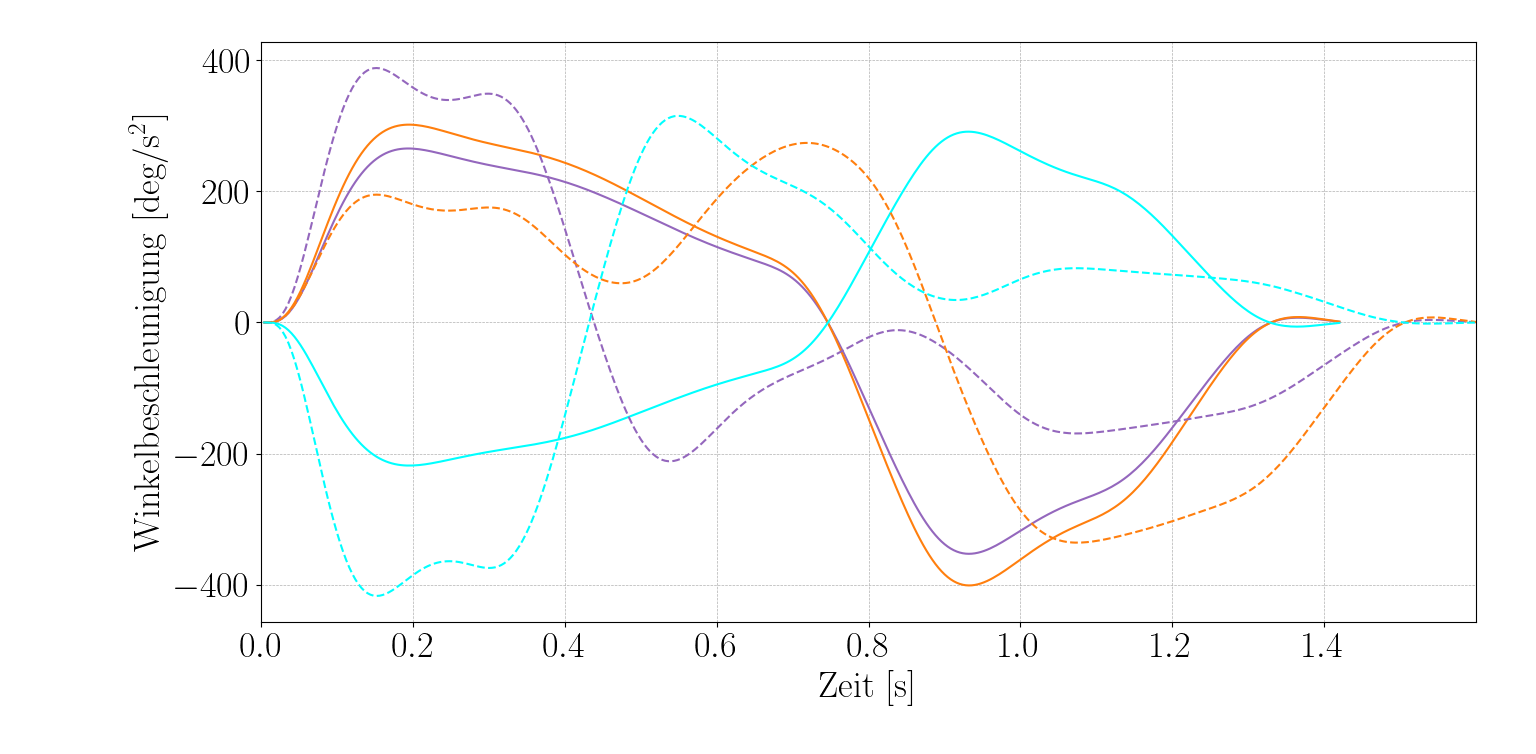
\includegraphics[width=1\linewidth]{images/accup2}
%	\caption{Winkelbeschleunigung in den Gelenken 4-6 Bewegung Zwei}
%	\label{fig:accup2}
%\end{figure}
%\subsection{Fehlerquellen}
%Temperatureinfluss auf die Reibung 